
\begin{frame}
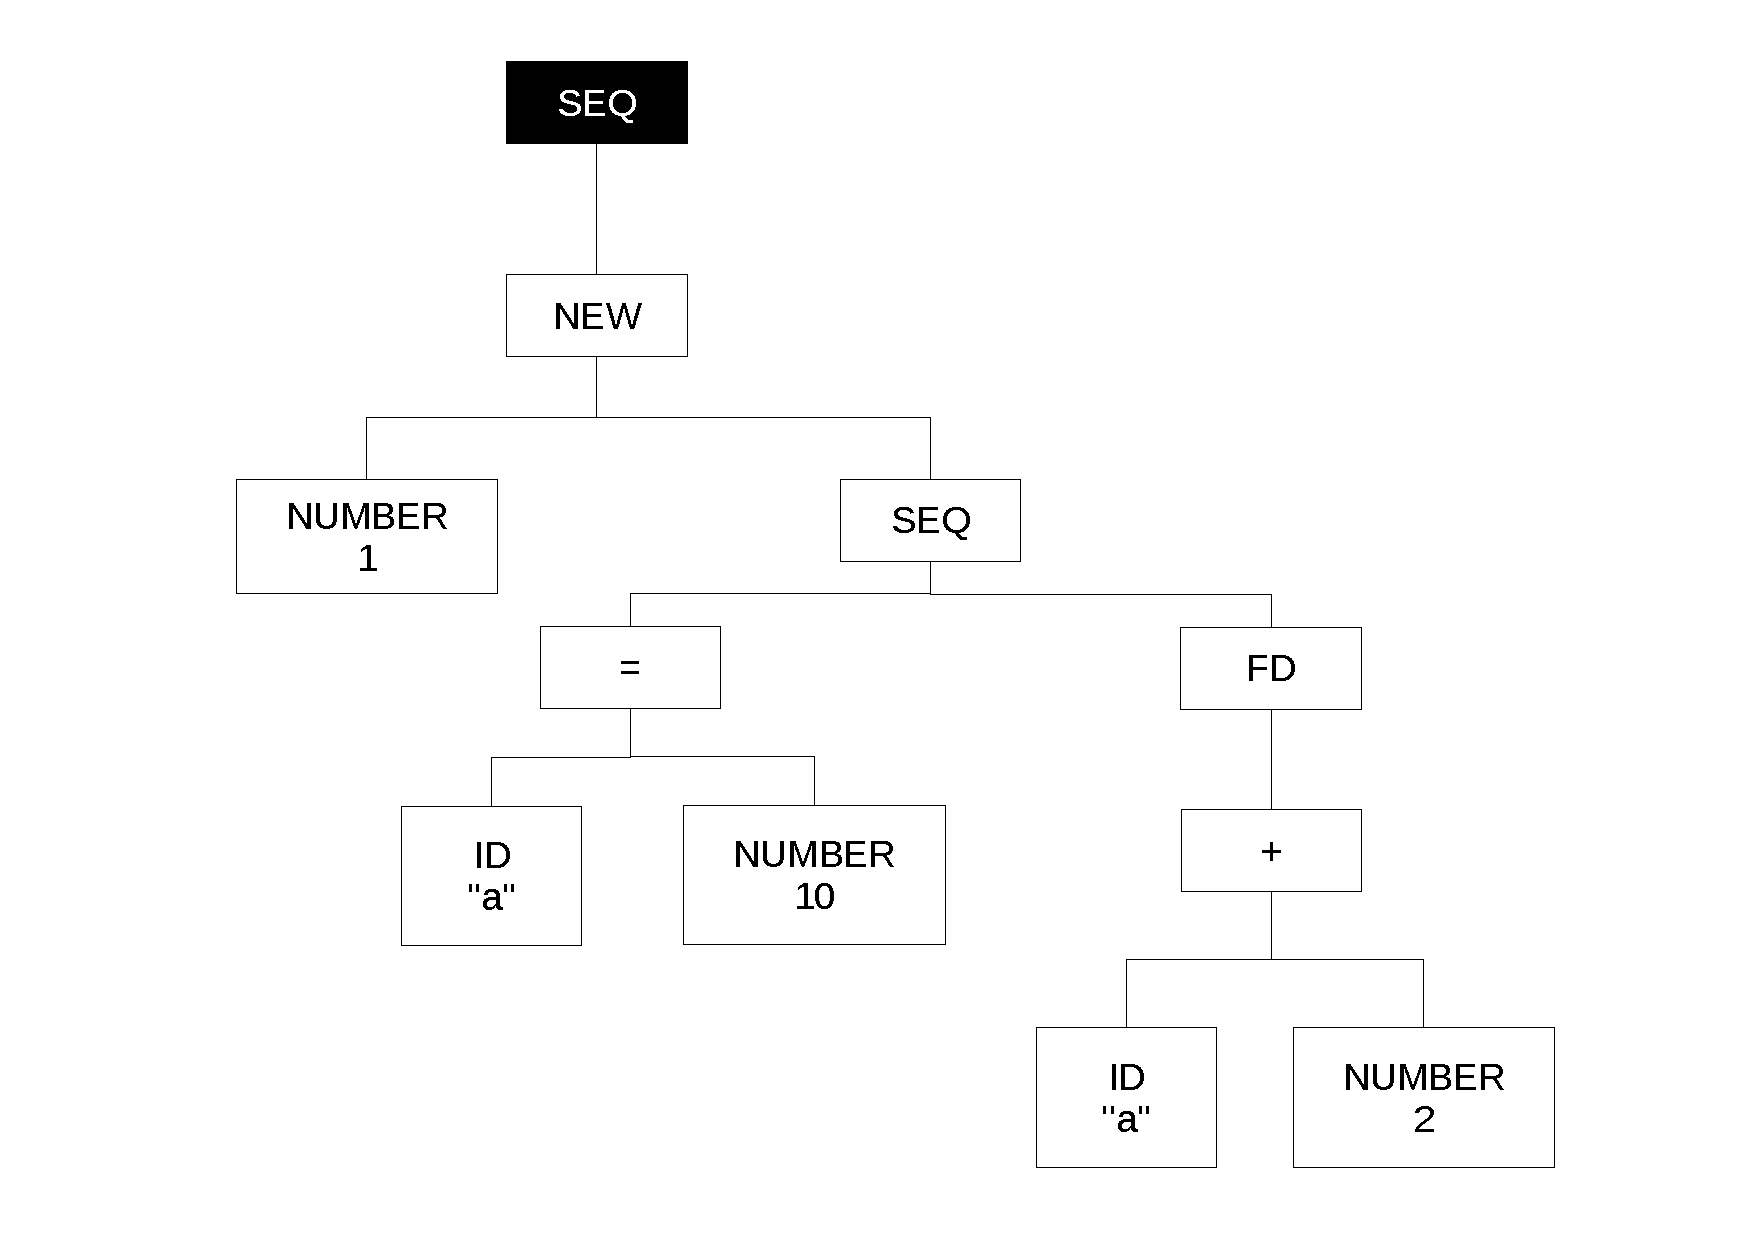
\includegraphics[scale=0.3]{doc/Presentation/img/arbre1.pdf}
\end{frame}

\begin{frame}
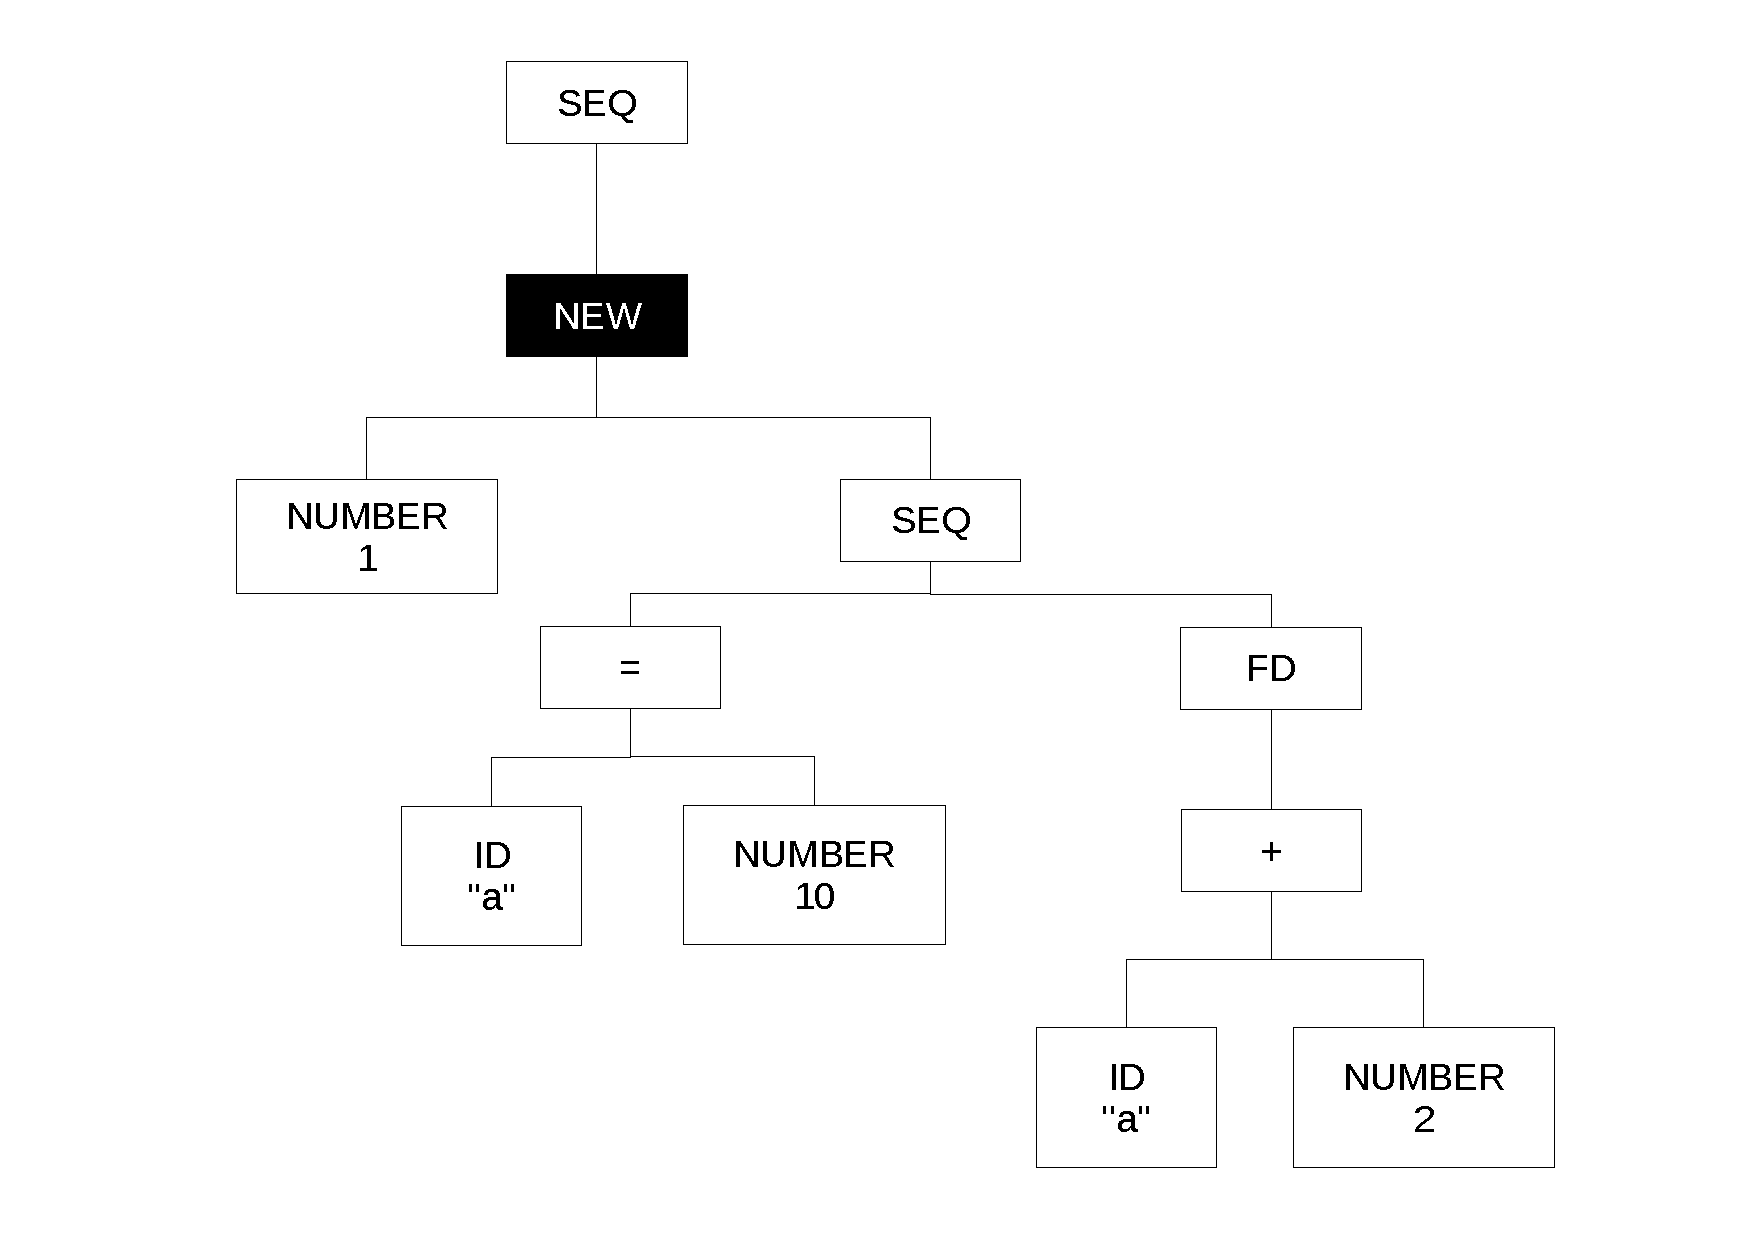
\includegraphics[scale=0.3]{doc/Presentation/img/arbre2.pdf}
\end{frame}

\begin{frame}[fragile]
	\begin{lstlisting}[language=Stibbons]
new agent {
  a = 10
  fd a + 2
}

1 new agent{
  a = 10
  fd a + 2
}
	\end{lstlisting}
\end{frame}

\begin{frame}
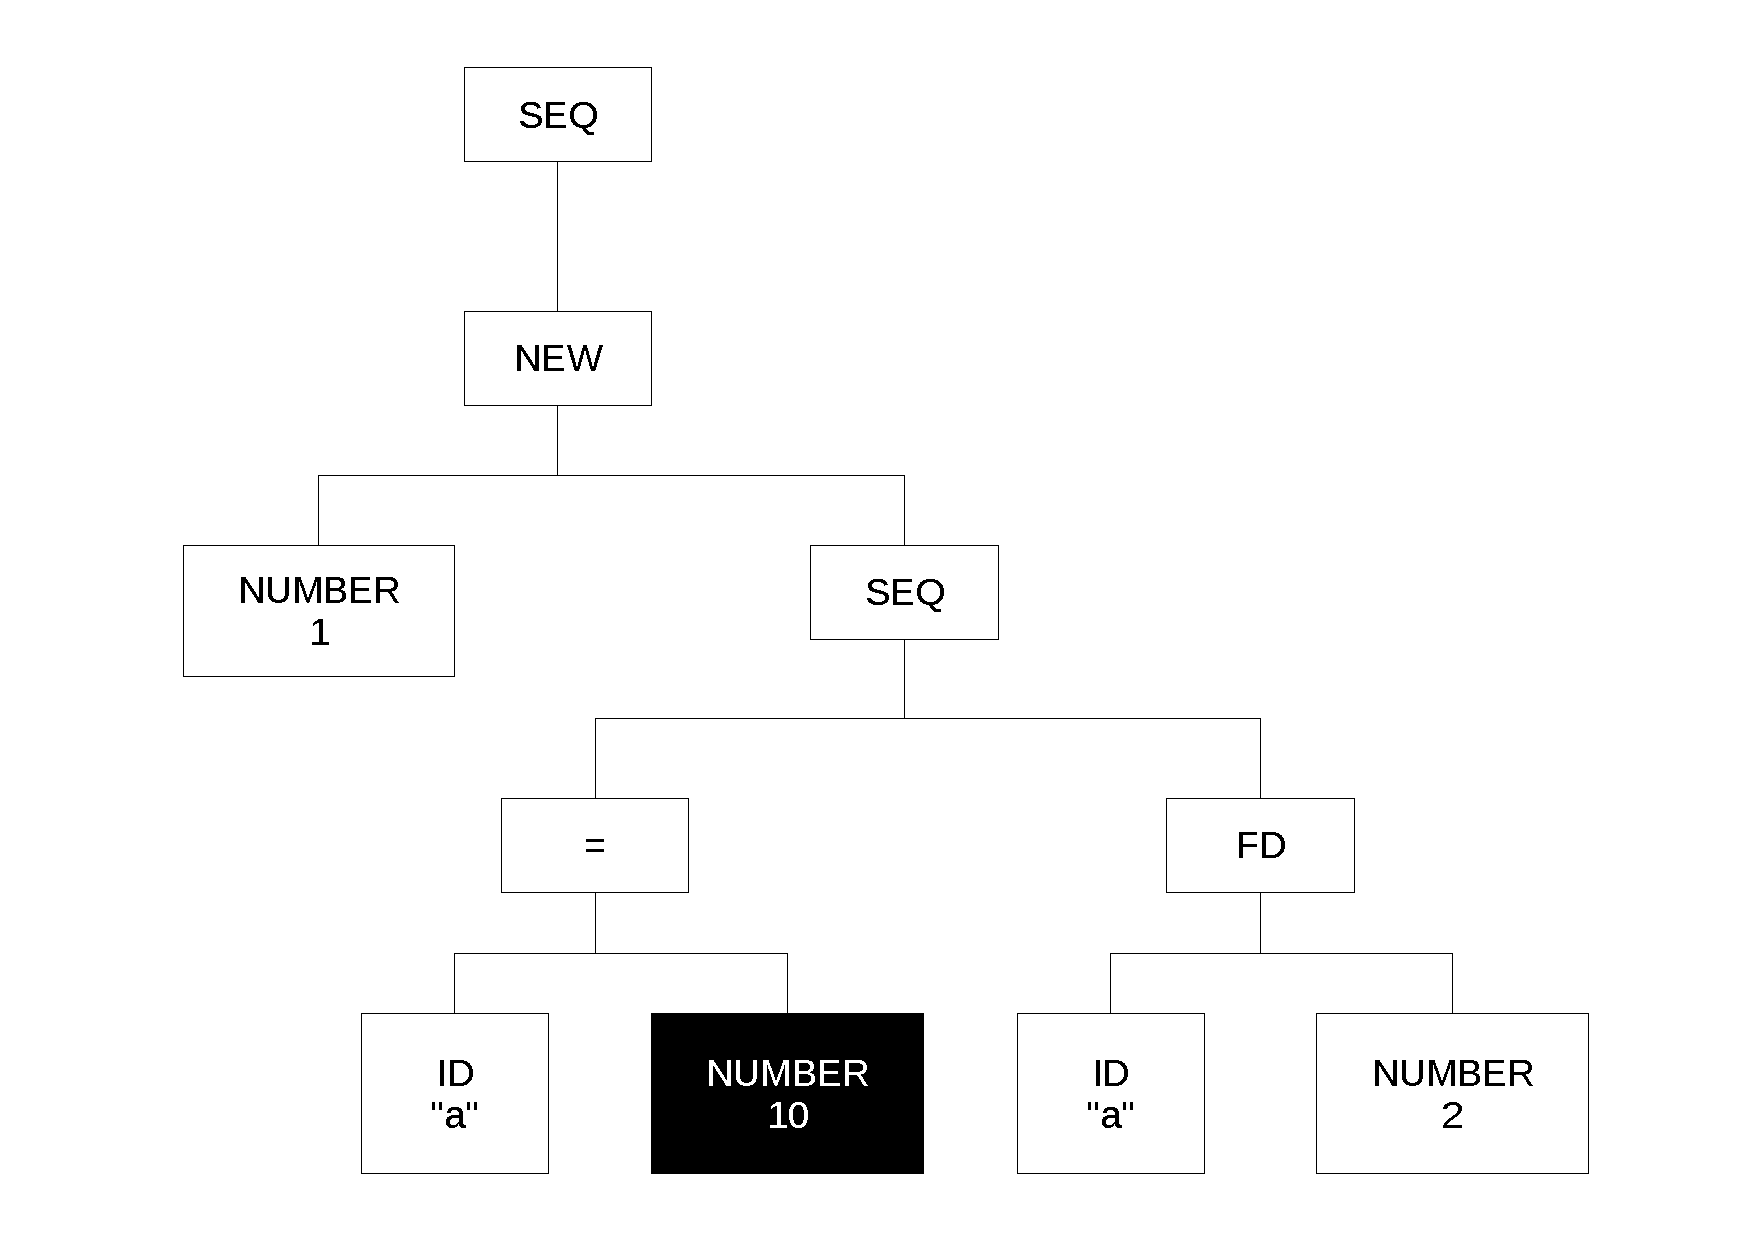
\includegraphics[scale=0.3]{doc/Presentation/img/arbre3.pdf}
\end{frame}

\begin{frame}
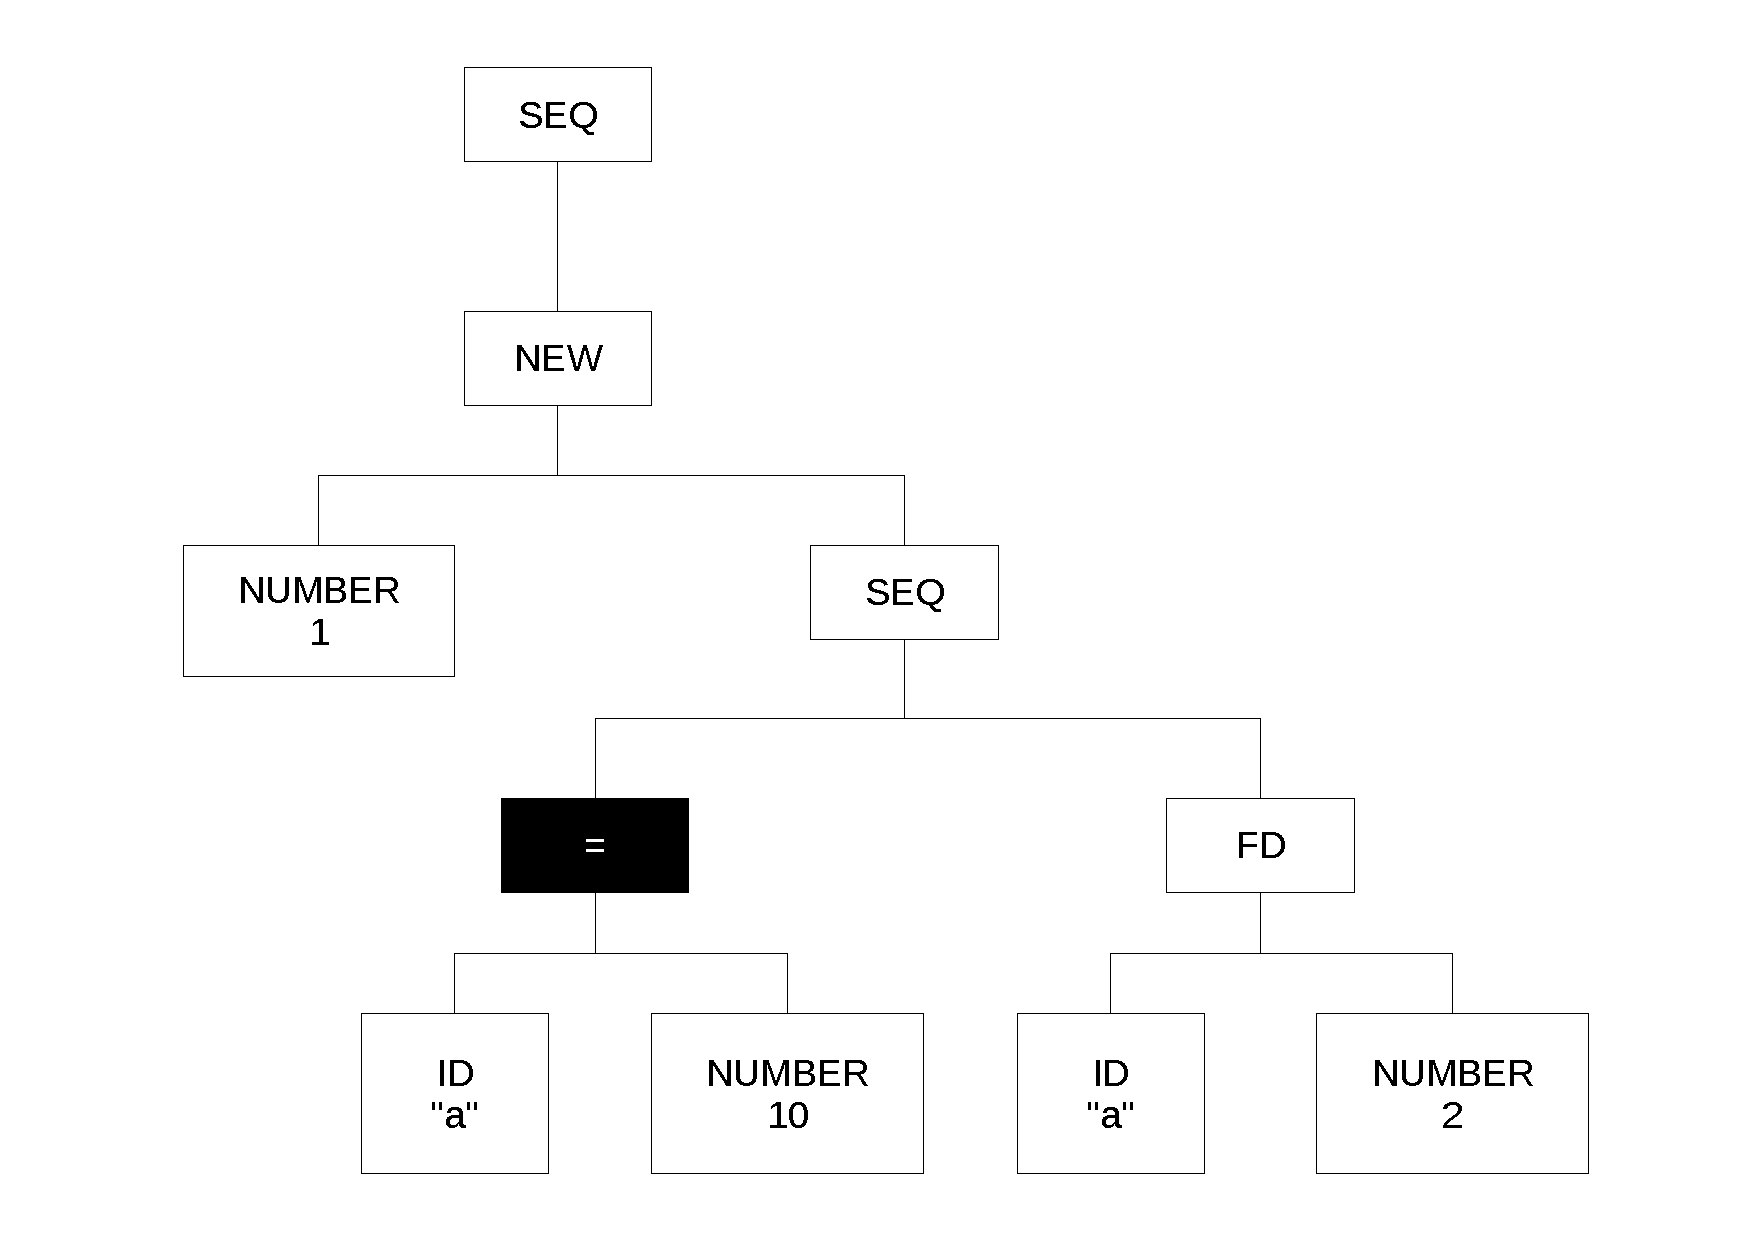
\includegraphics[scale=0.3]{doc/Presentation/img/arbre4.pdf}
\end{frame}

\begin{frame}
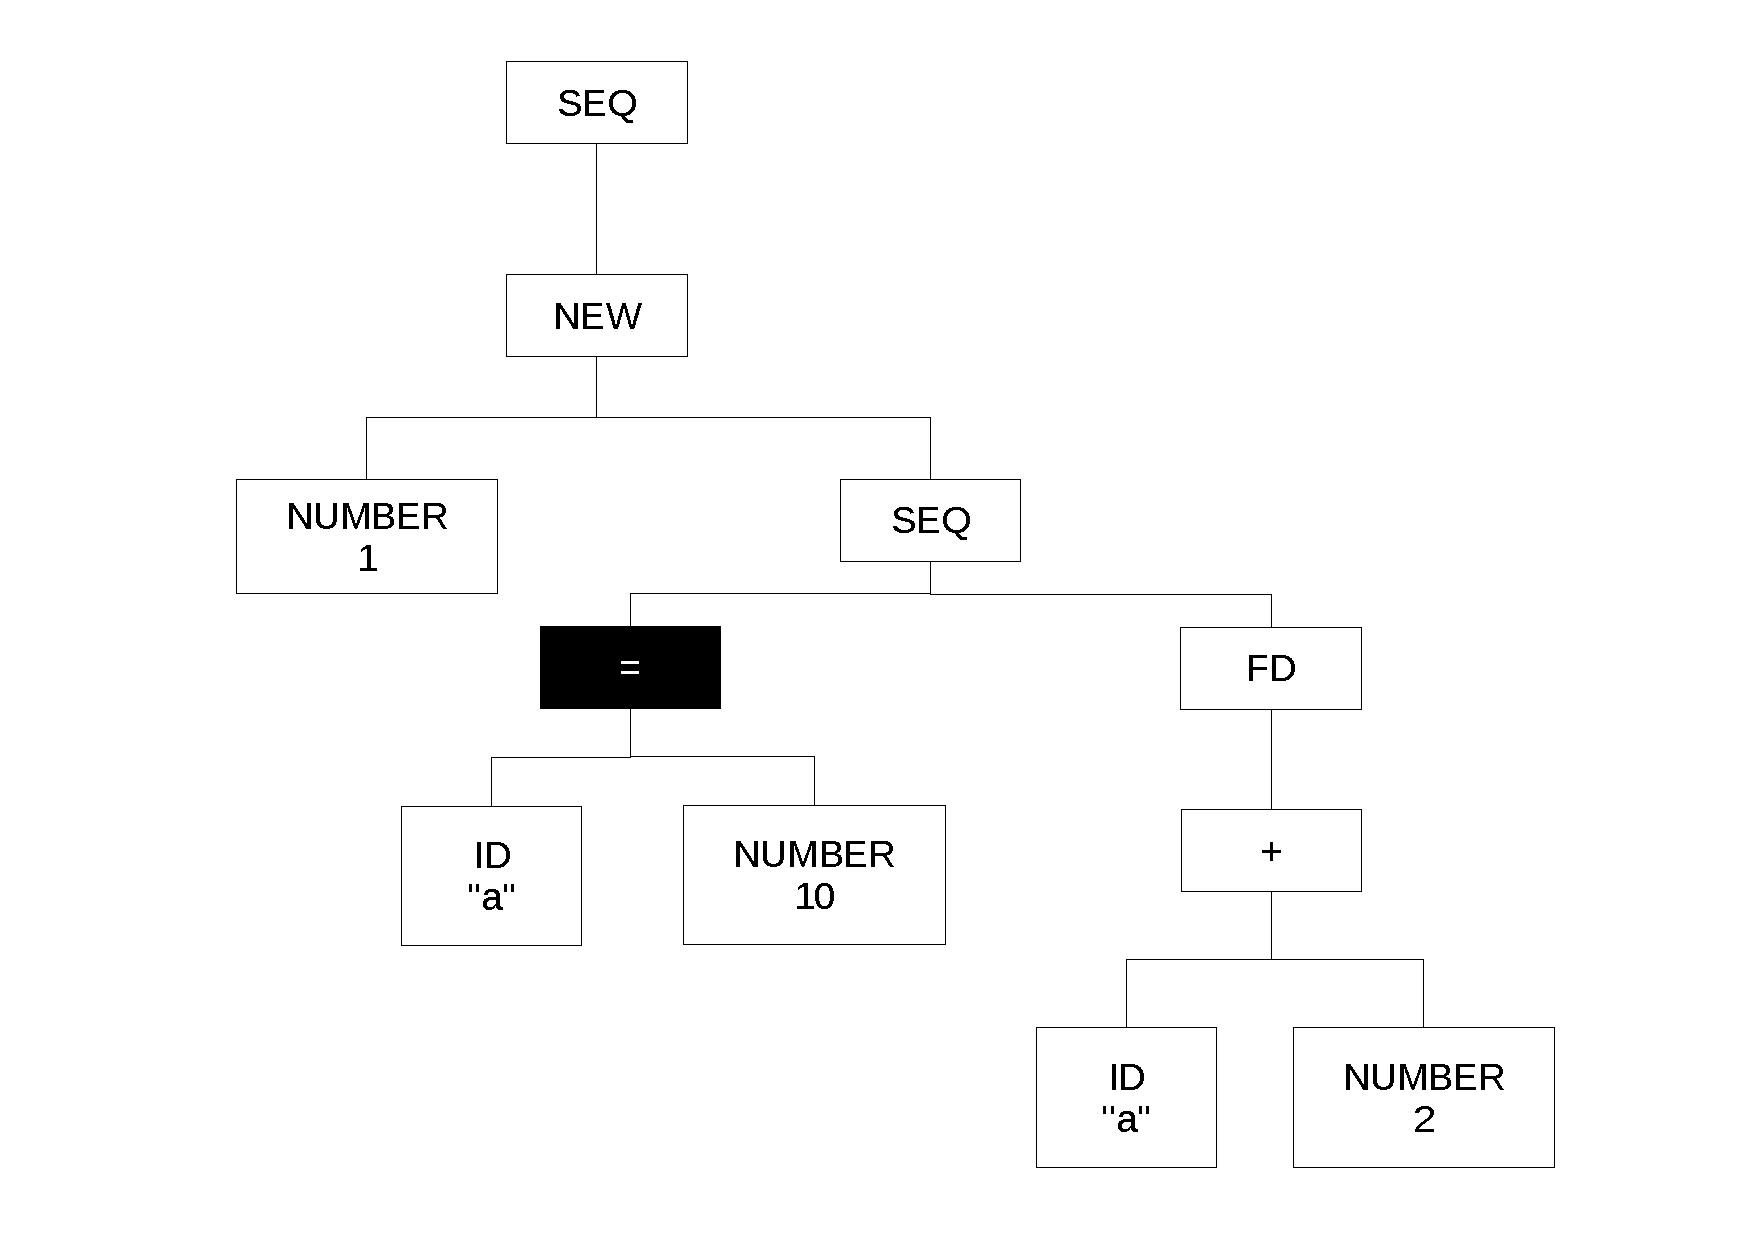
\includegraphics[scale=0.3]{doc/Presentation/img/arbre5.pdf}
\end{frame}

\begin{frame}
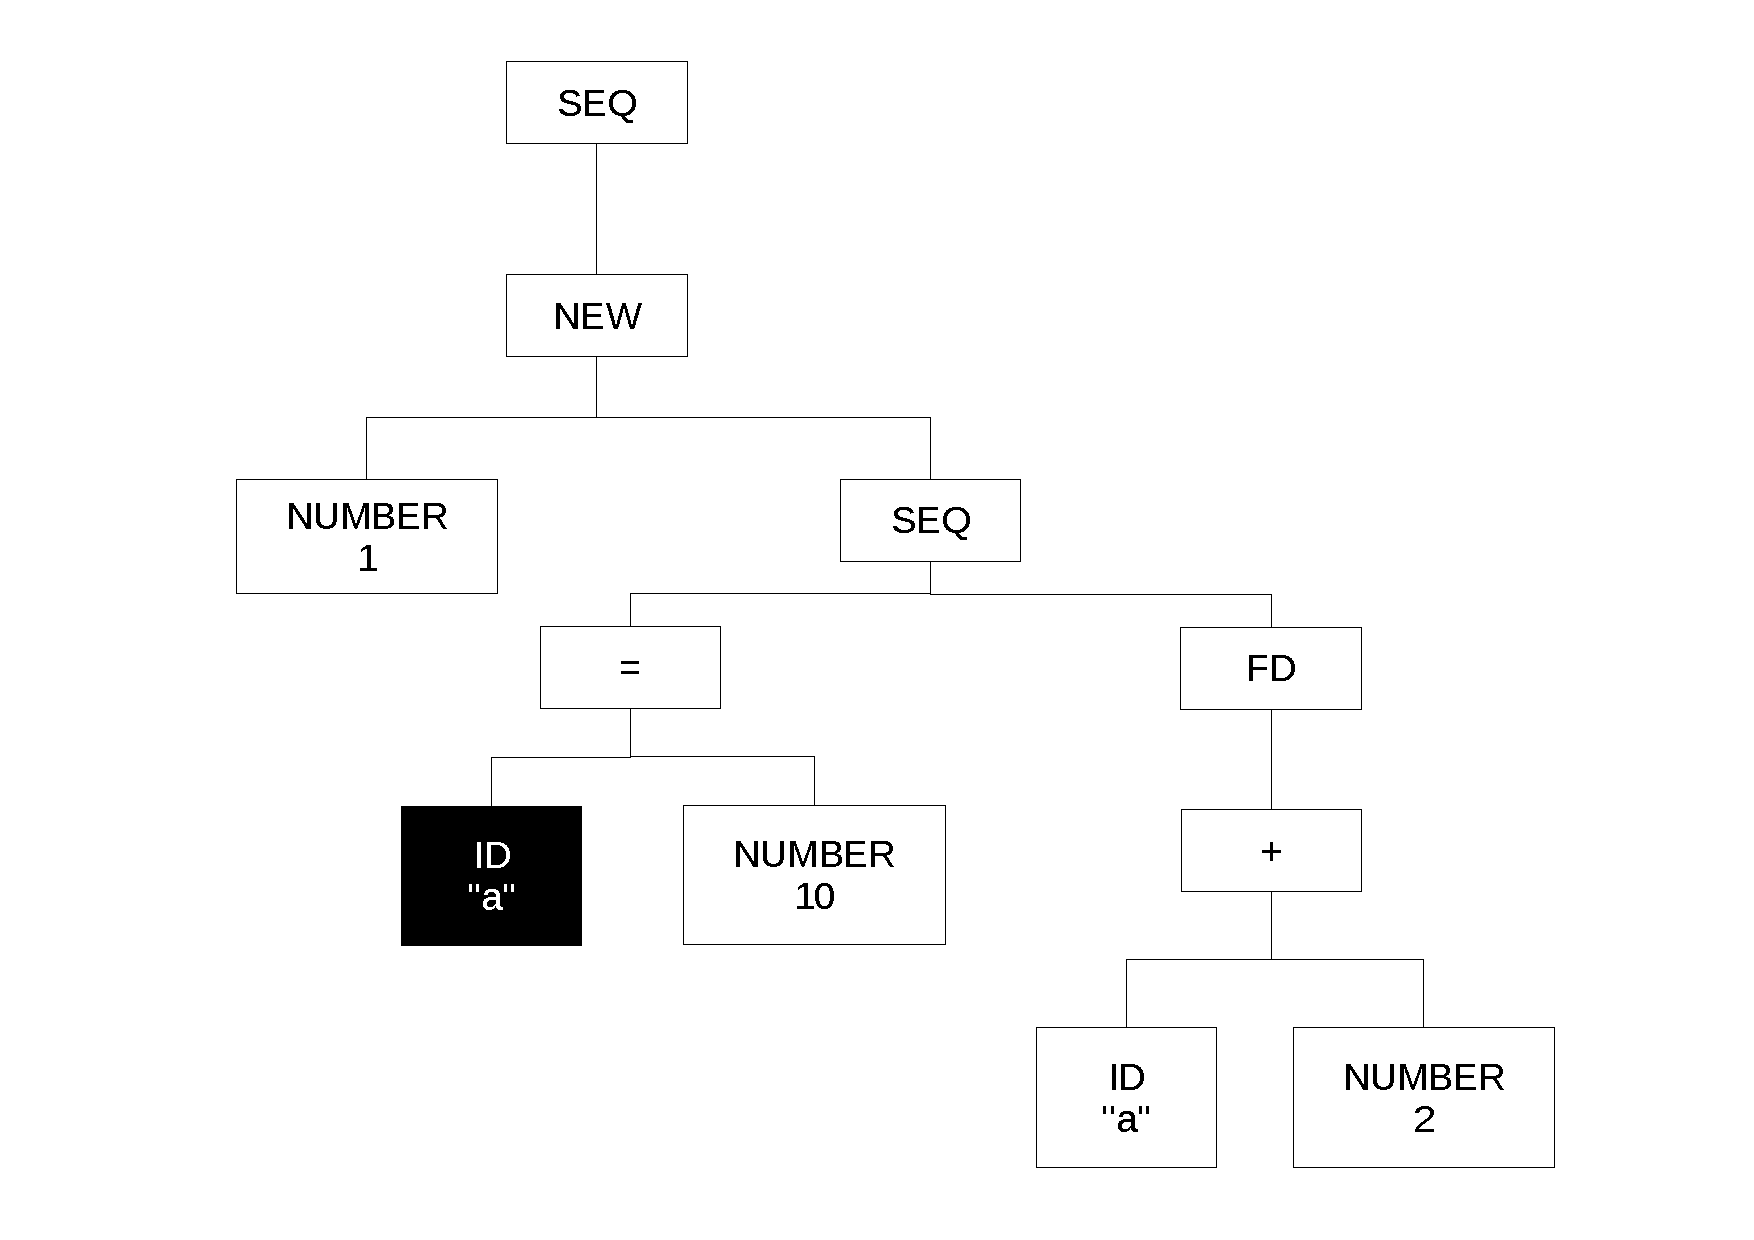
\includegraphics[scale=0.3]{doc/Presentation/img/arbre6.pdf}
\end{frame}

\begin{frame}
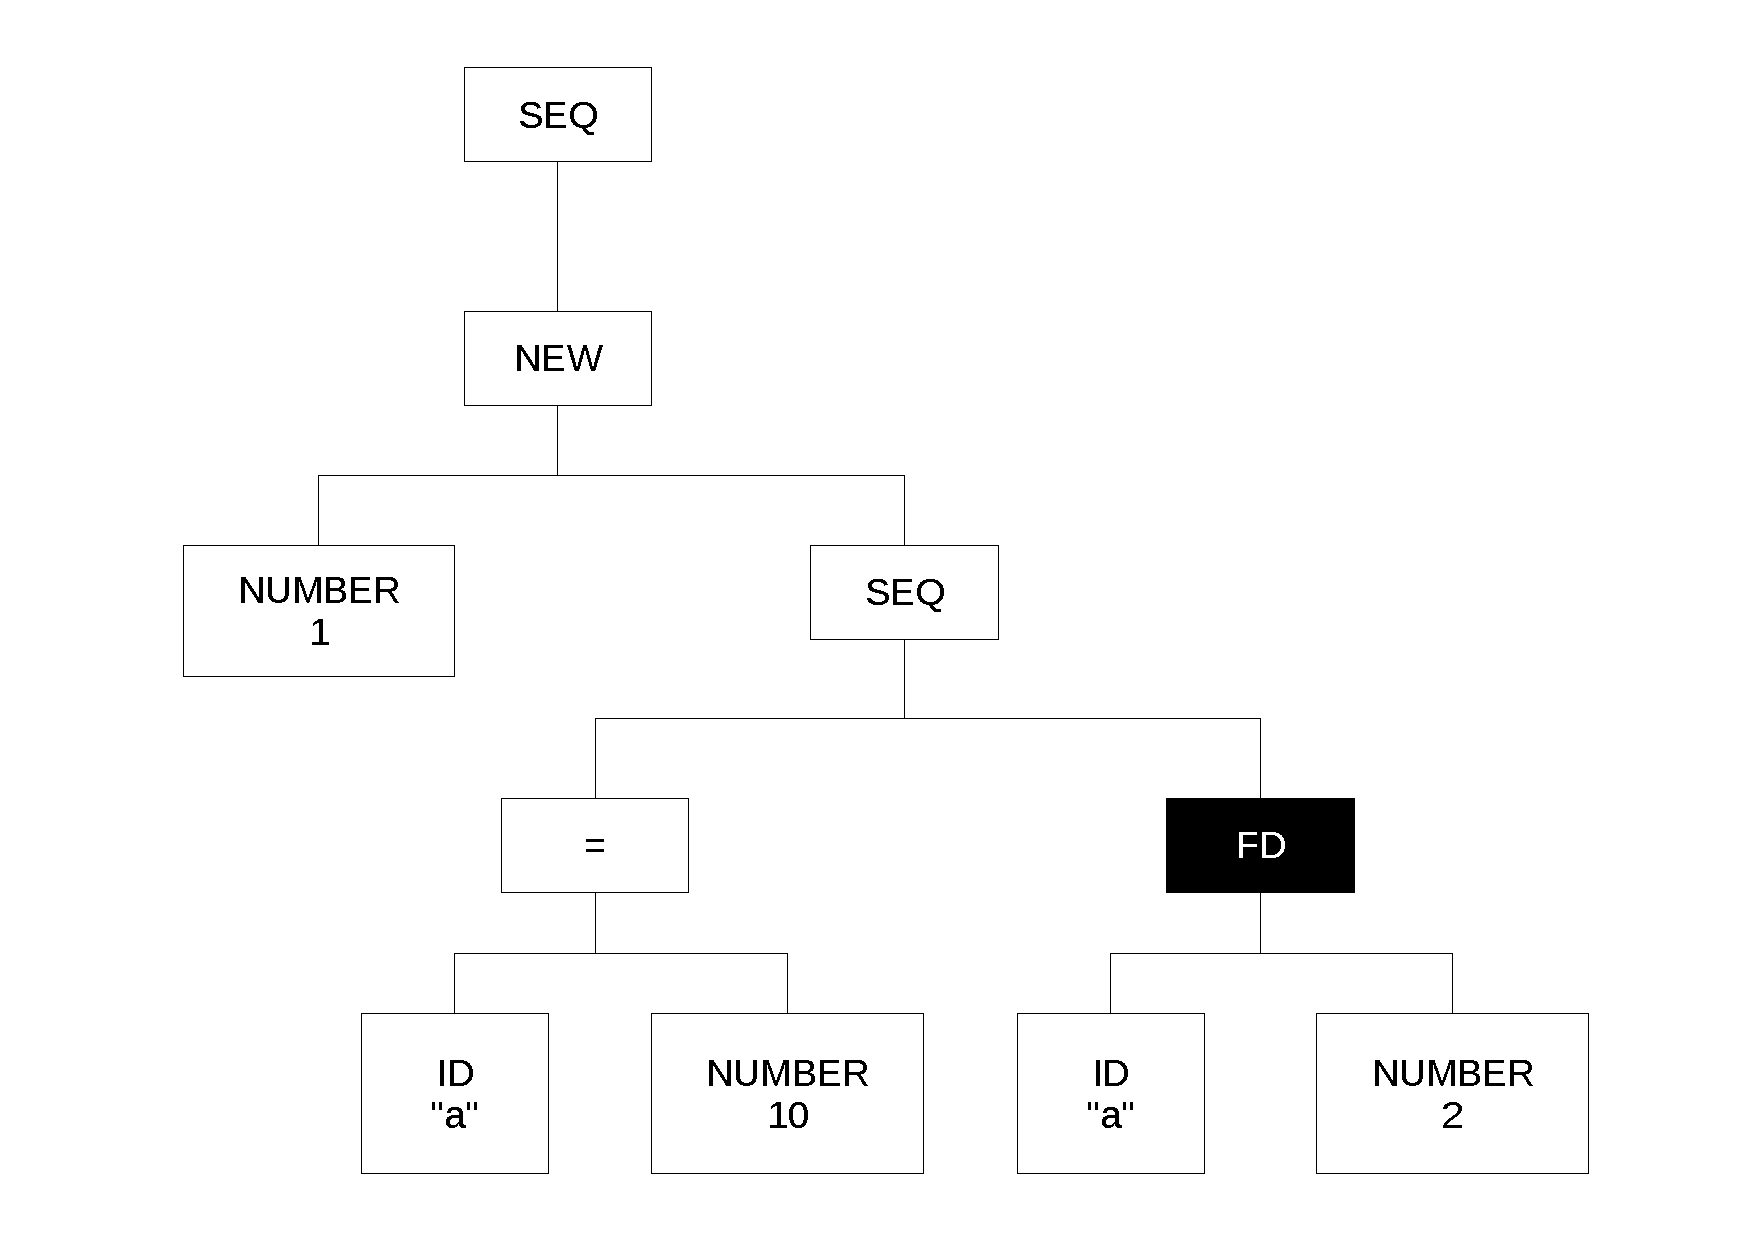
\includegraphics[scale=0.3]{doc/Presentation/img/arbre7.pdf}
\end{frame}

\begin{frame}
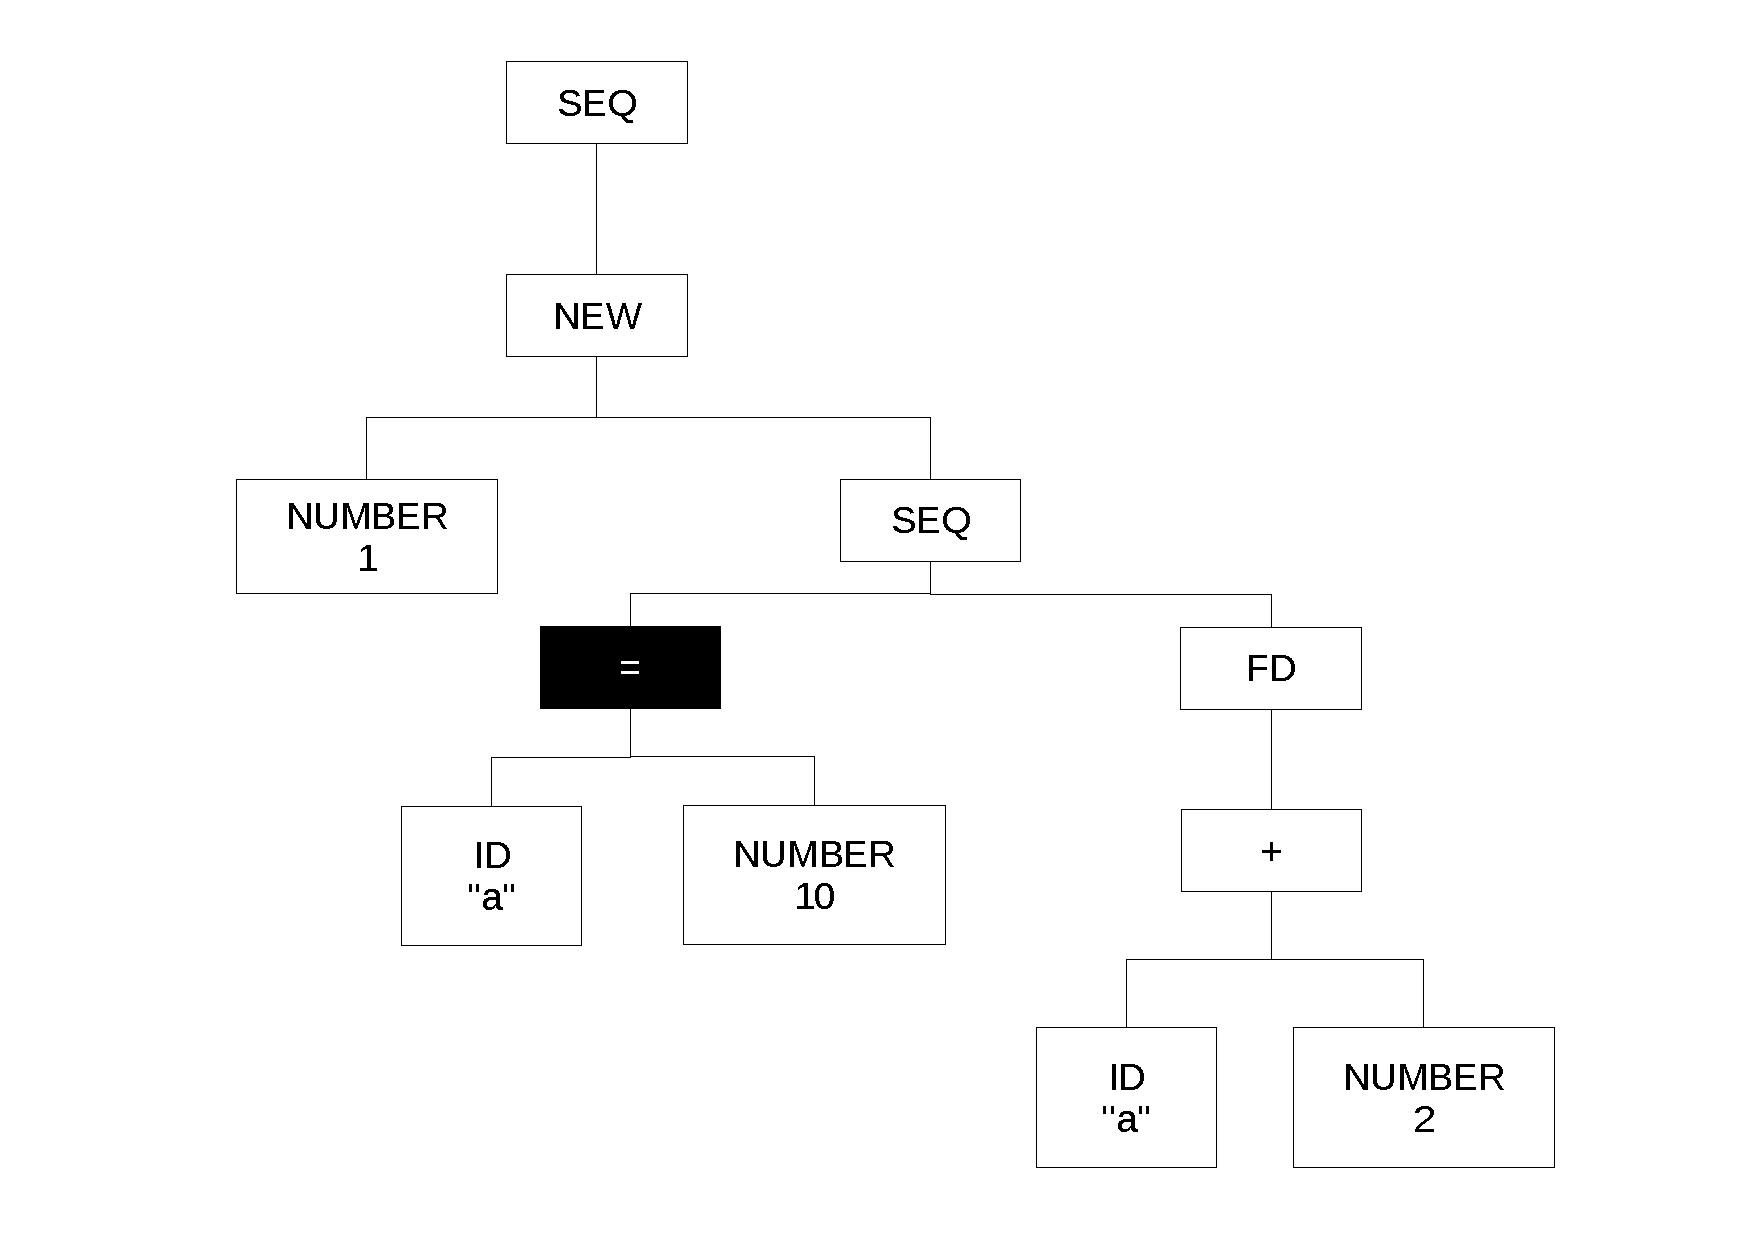
\includegraphics[scale=0.3]{doc/Presentation/img/arbre5.pdf}
\end{frame}

\begin{frame}
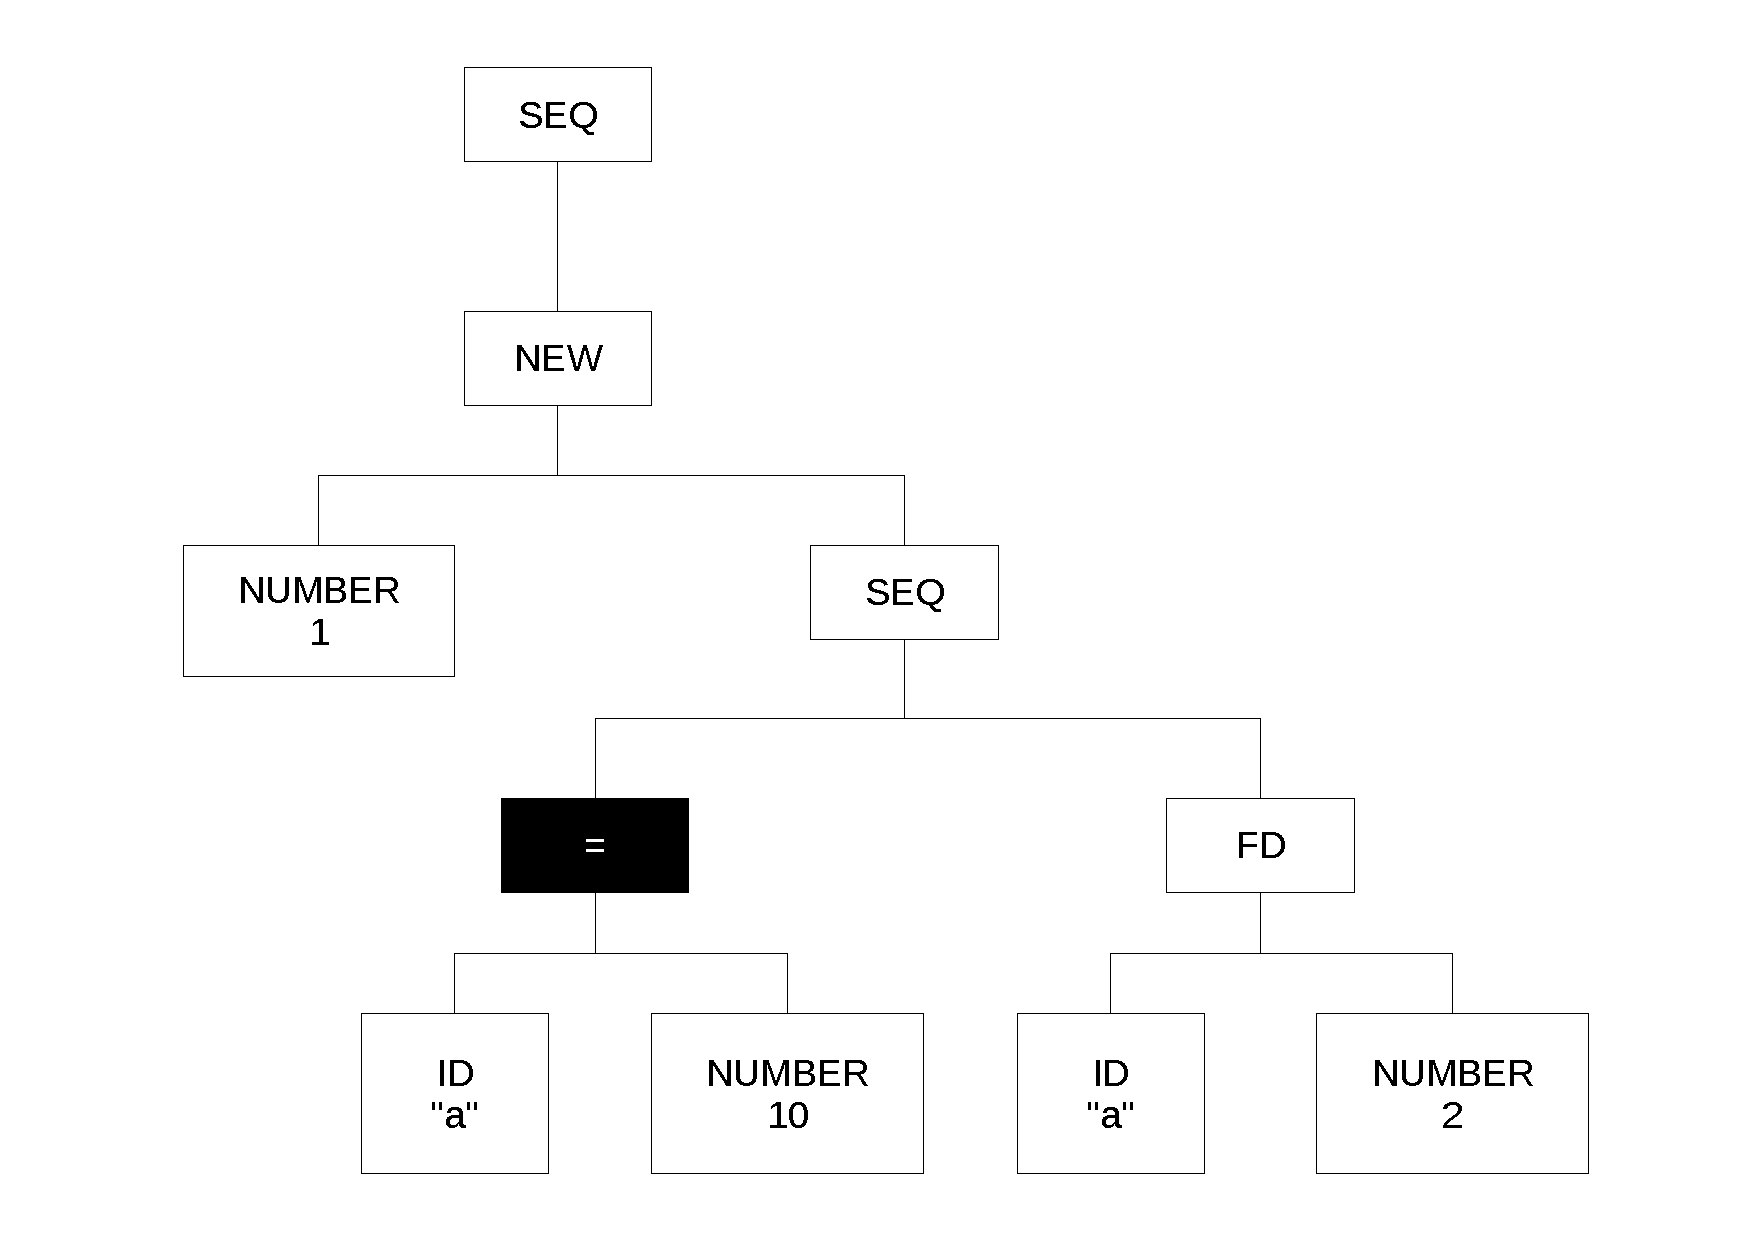
\includegraphics[scale=0.3]{doc/Presentation/img/arbre4.pdf}
\end{frame}

\begin{frame}
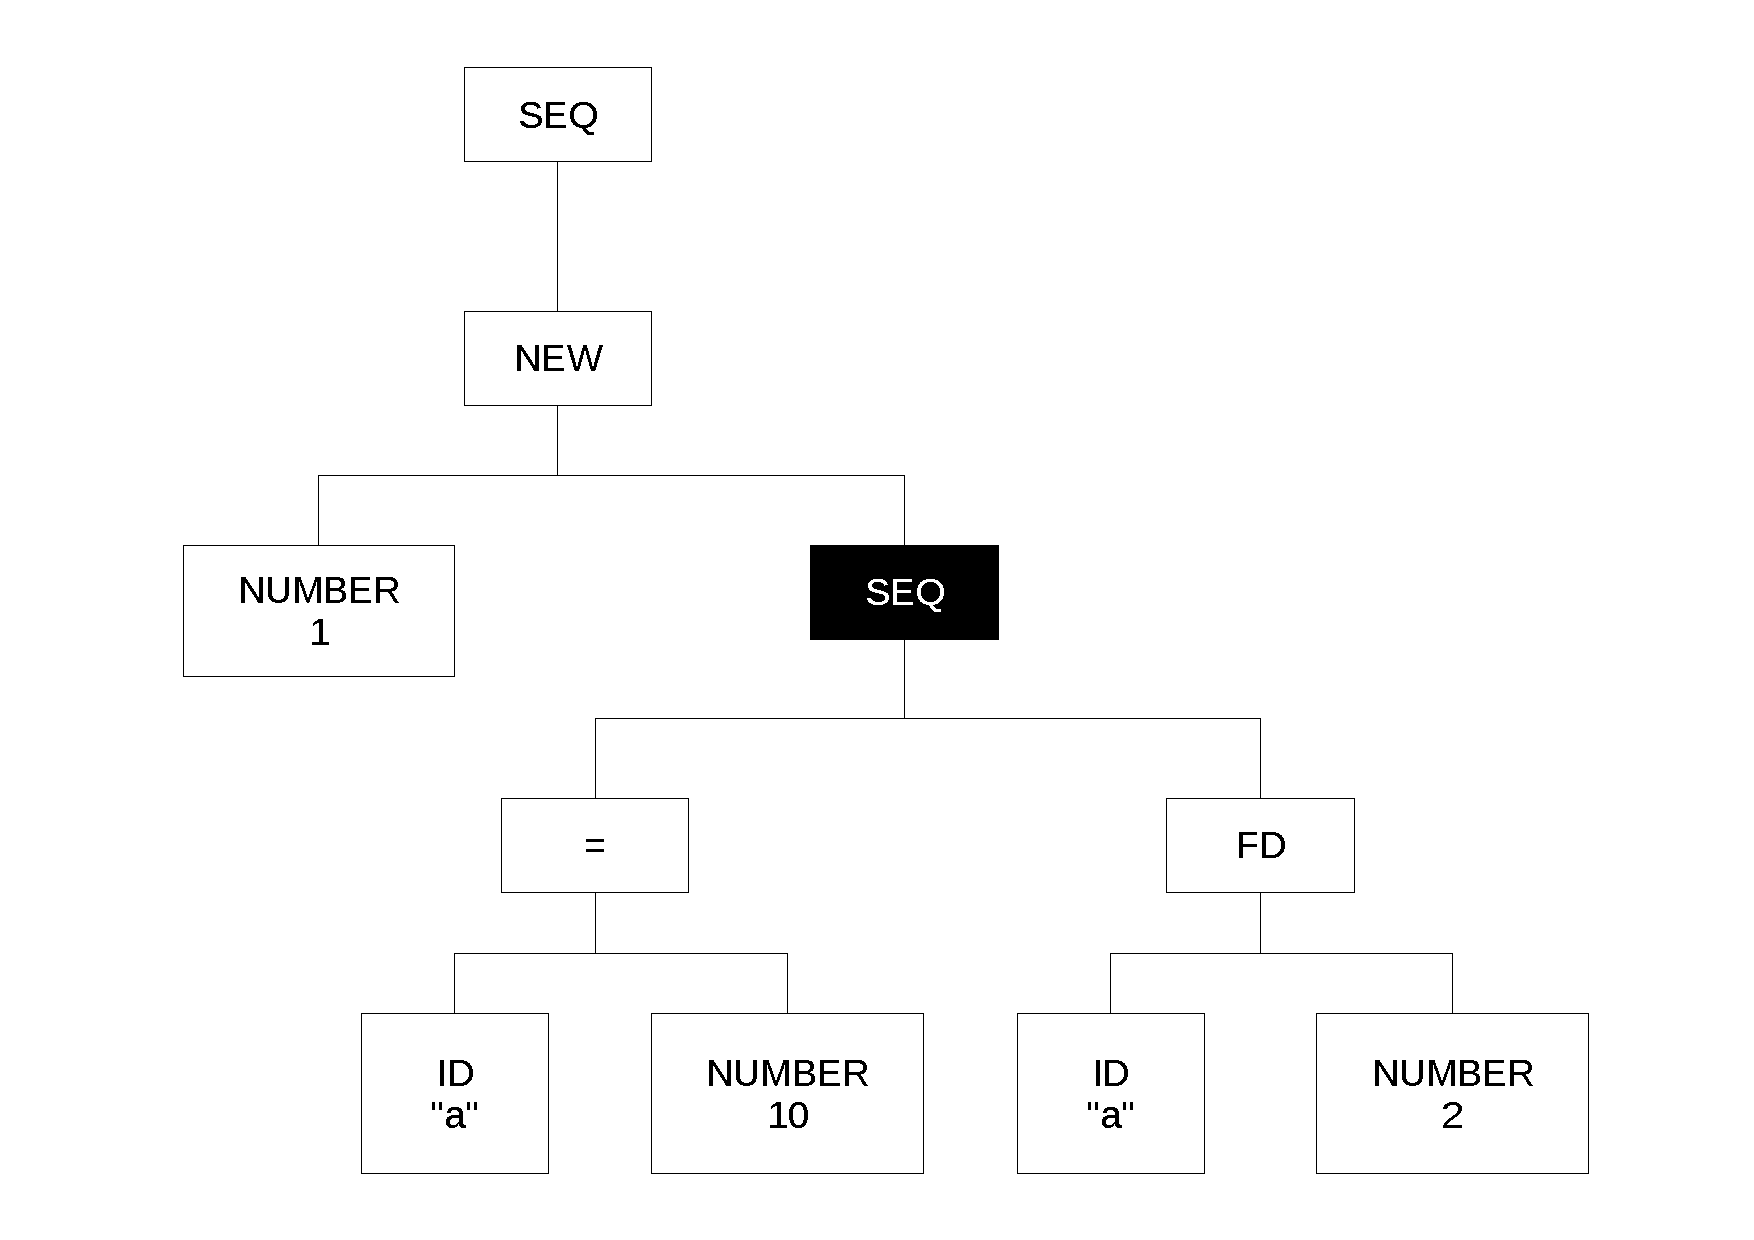
\includegraphics[scale=0.3]{doc/Presentation/img/arbre8.pdf}
\end{frame}

\begin{frame}
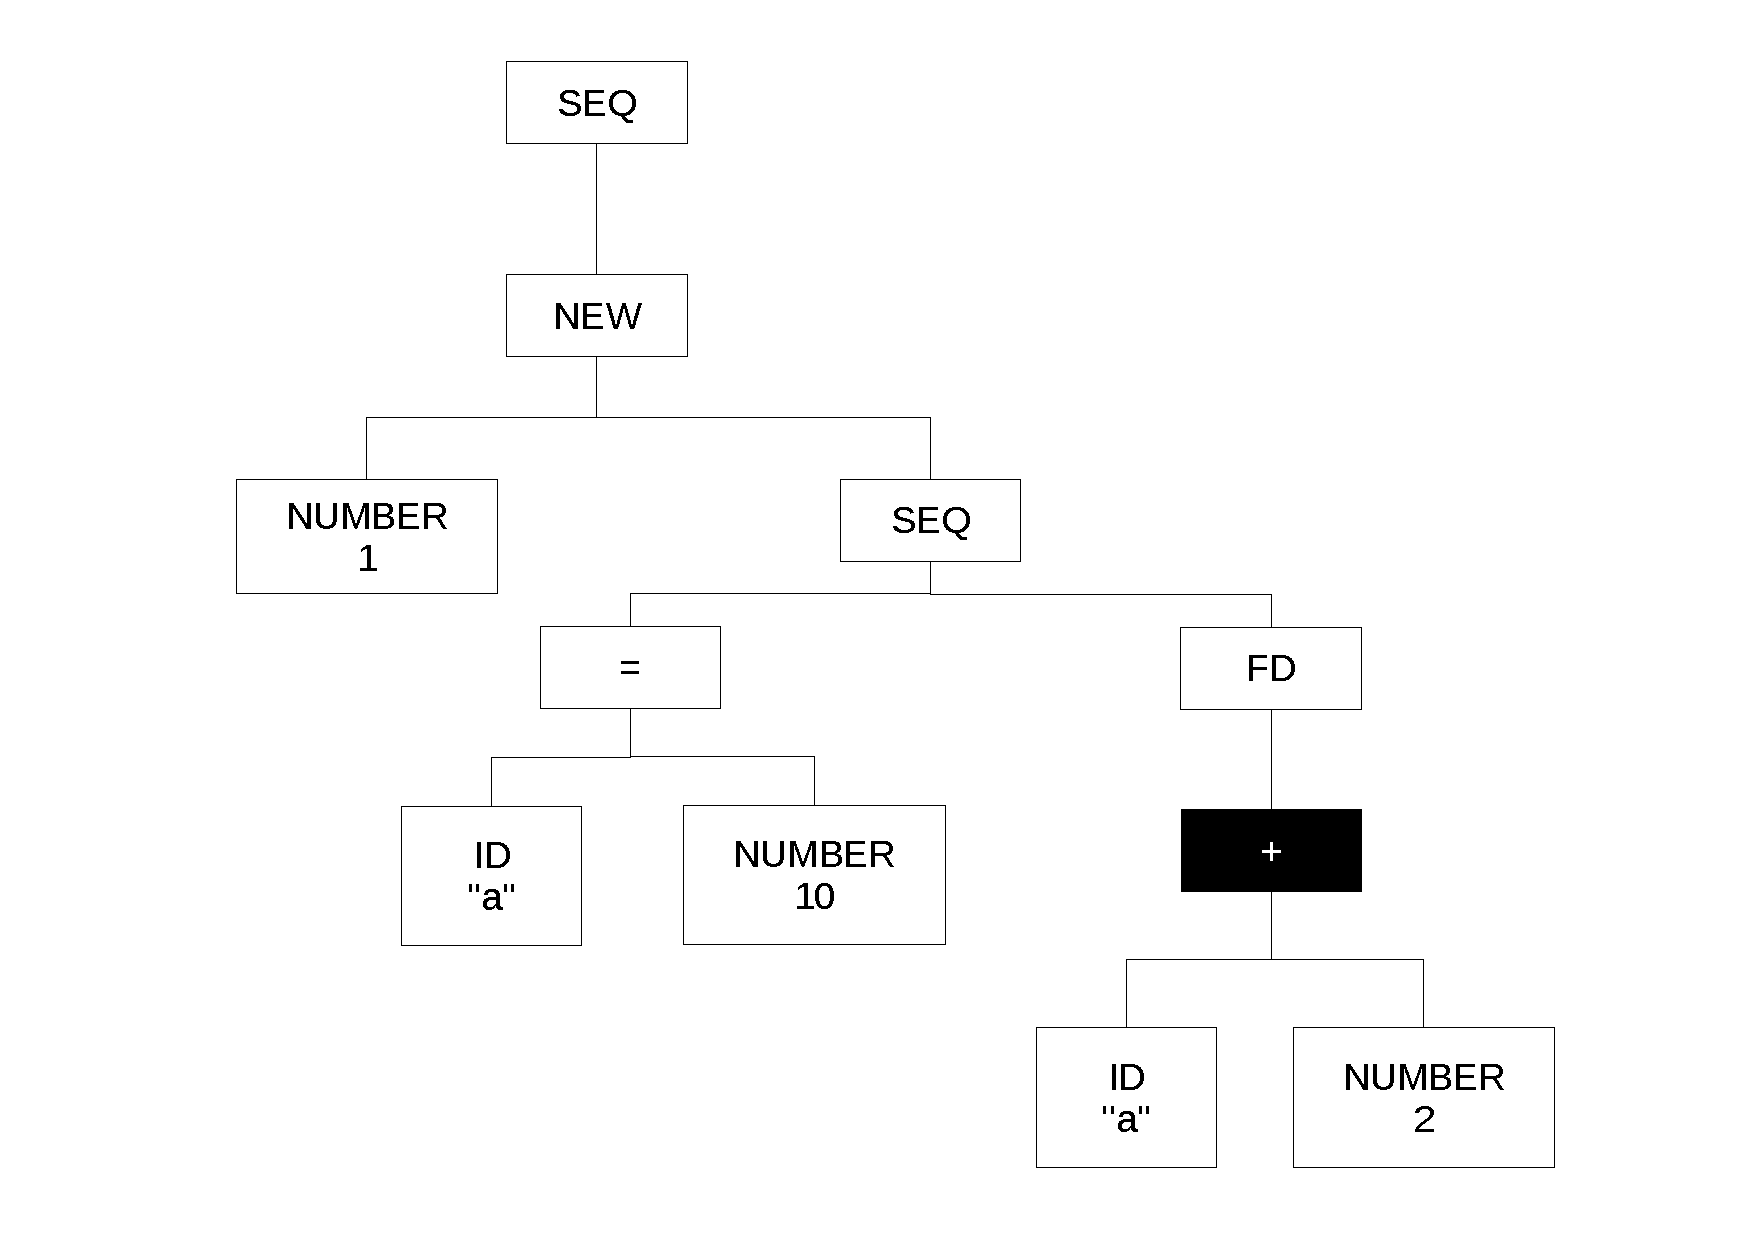
\includegraphics[scale=0.3]{doc/Presentation/img/arbre9.pdf}
\end{frame}

\begin{frame}
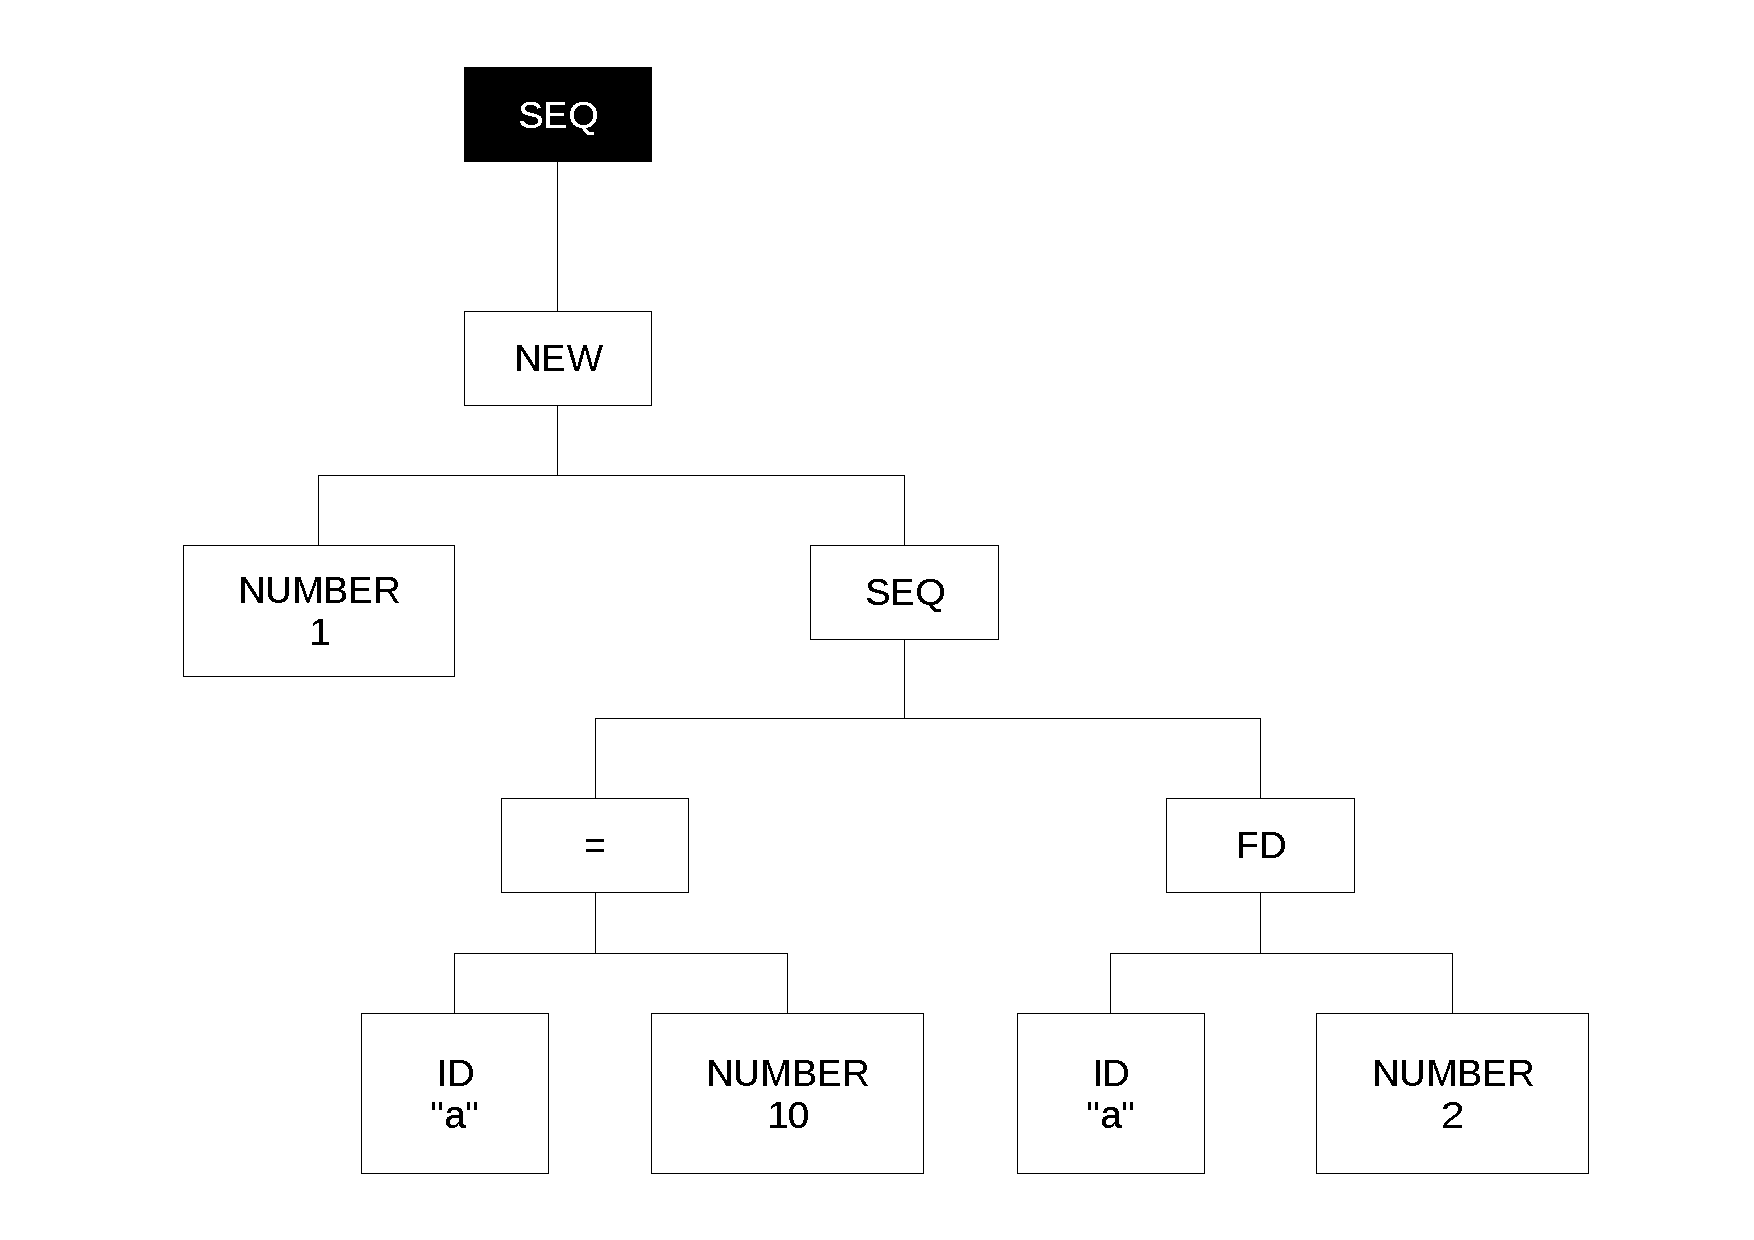
\includegraphics[scale=0.3]{doc/Presentation/img/arbre10.pdf}
\end{frame}

\begin{frame}
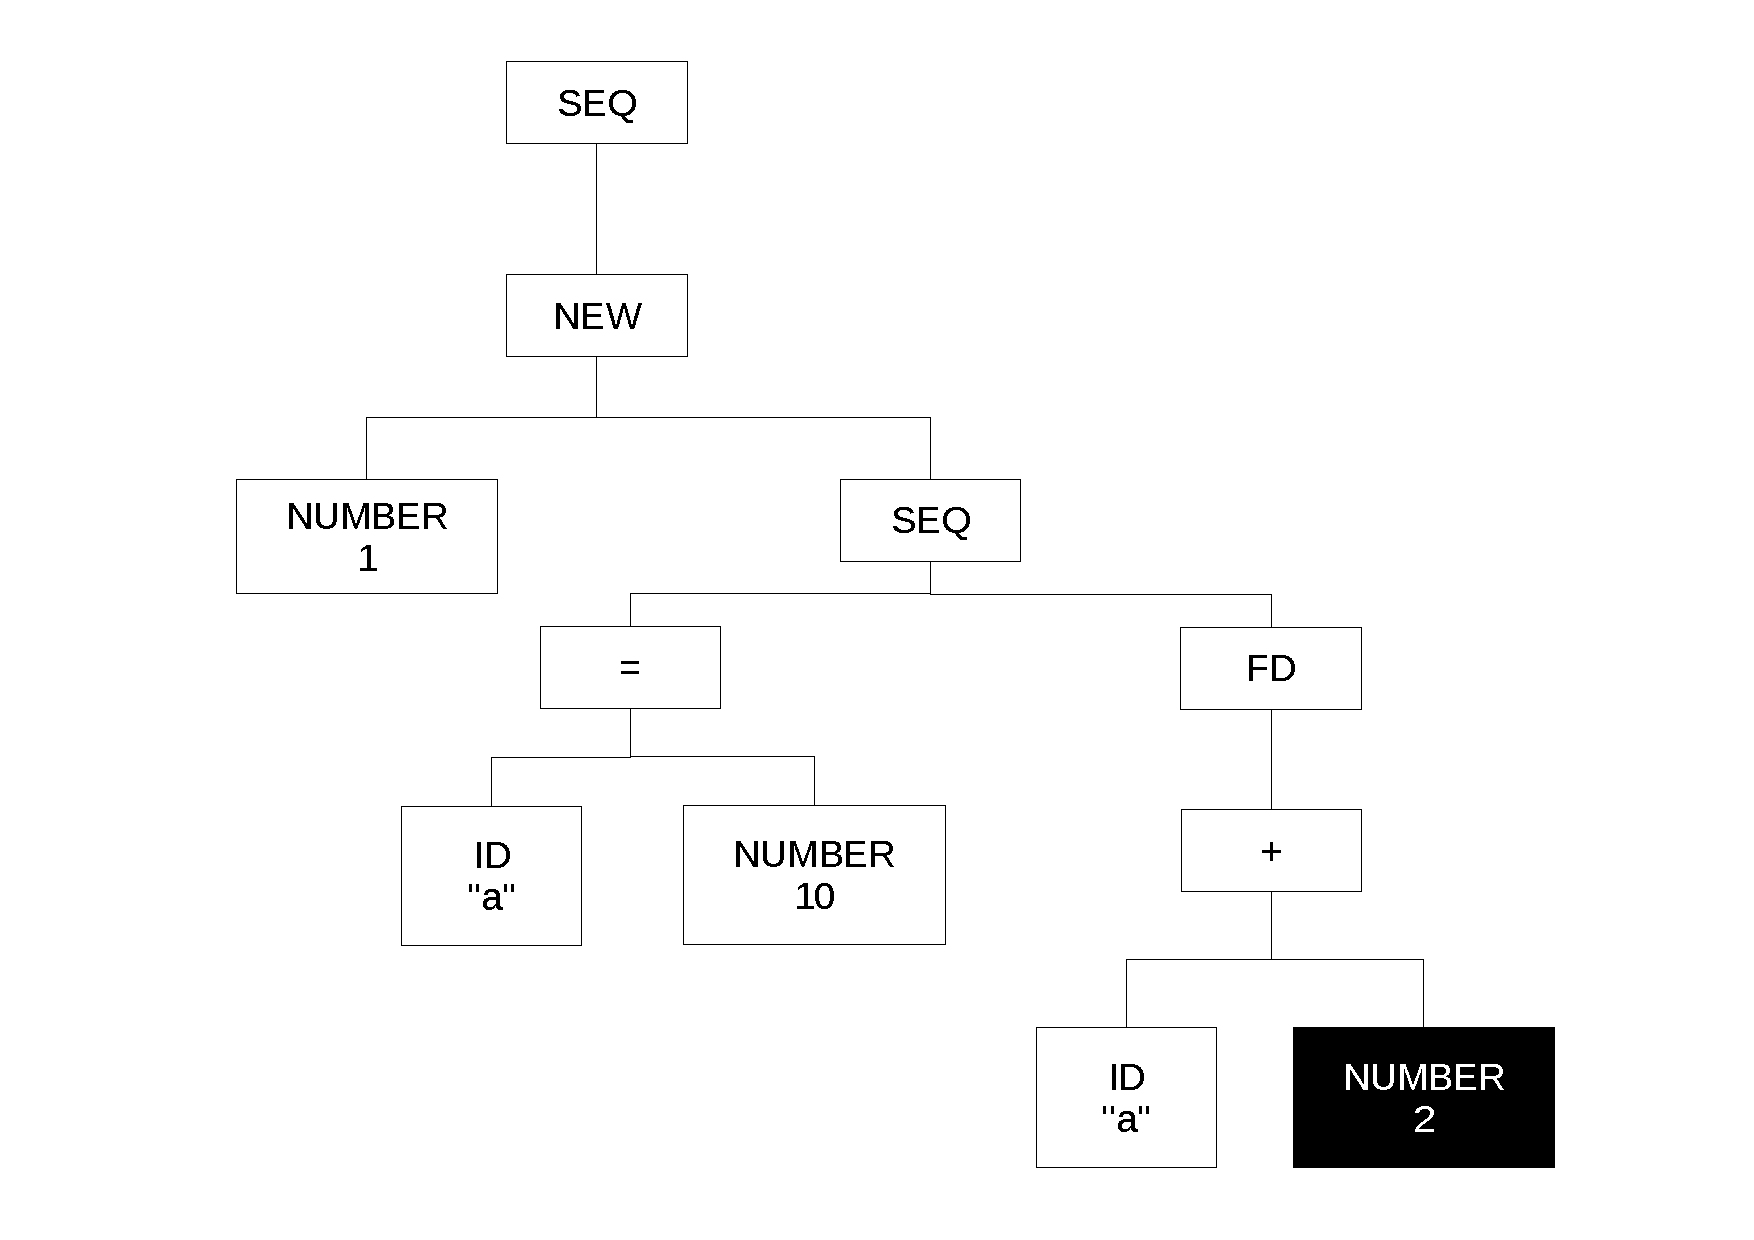
\includegraphics[scale=0.3]{doc/Presentation/img/arbre11.pdf}
\end{frame}

\begin{frame}
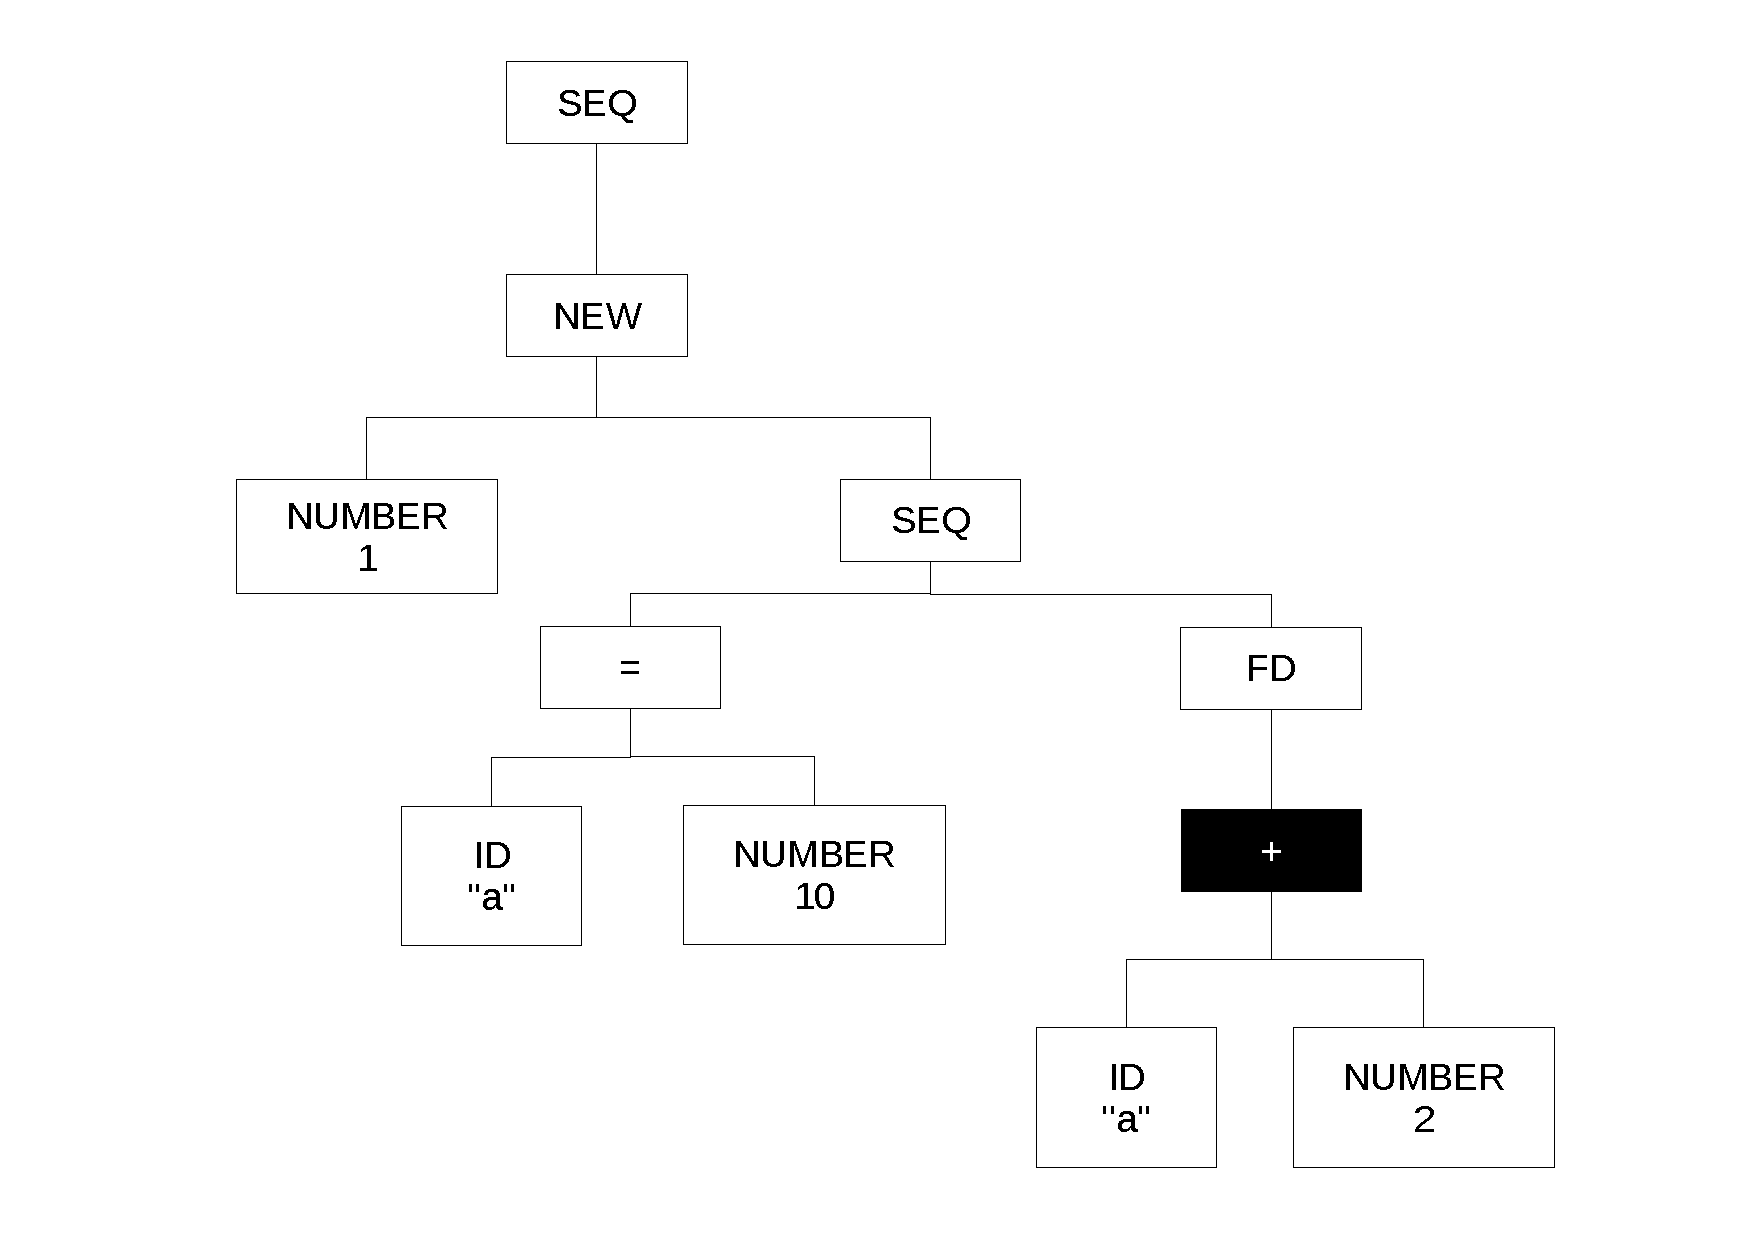
\includegraphics[scale=0.3]{doc/Presentation/img/arbre9.pdf}
\end{frame}

\begin{frame}
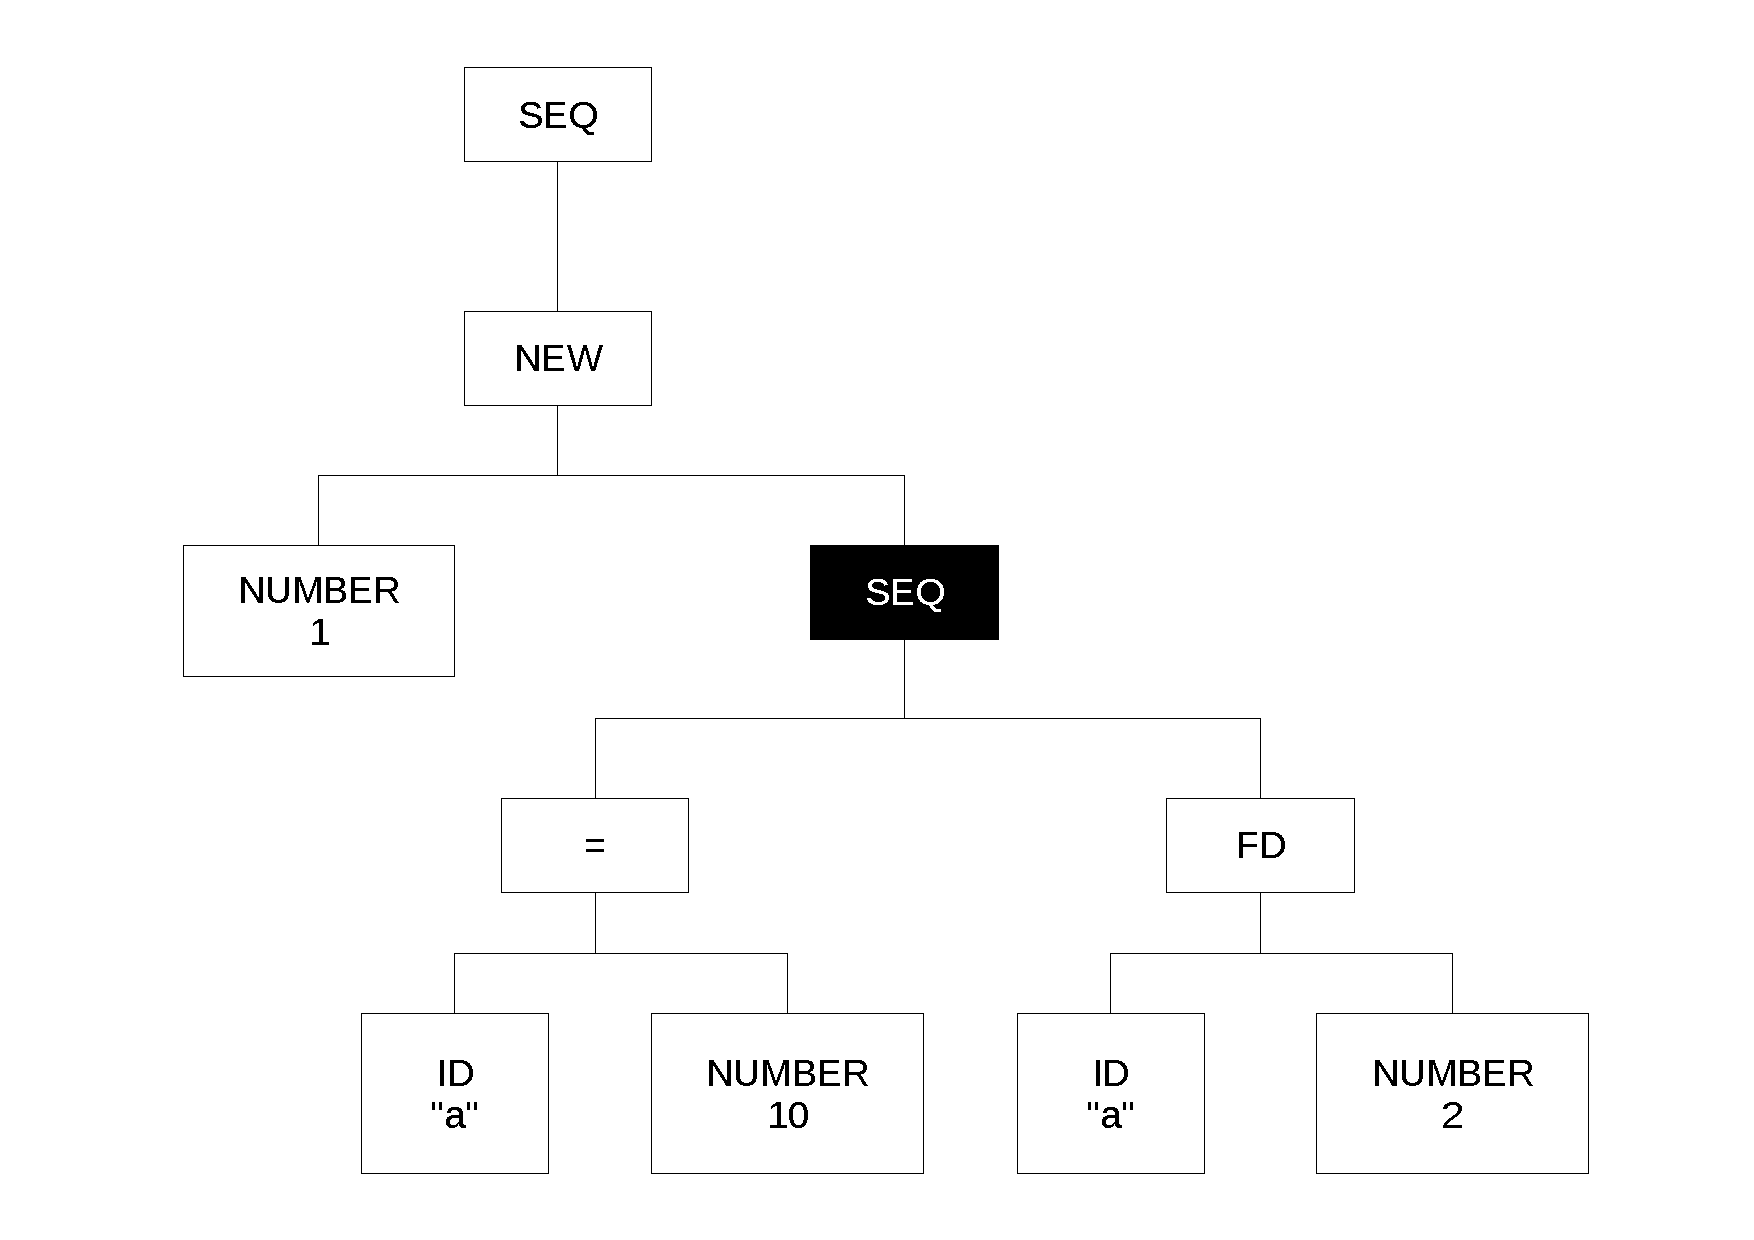
\includegraphics[scale=0.3]{doc/Presentation/img/arbre8.pdf}
\end{frame}

\begin{frame}
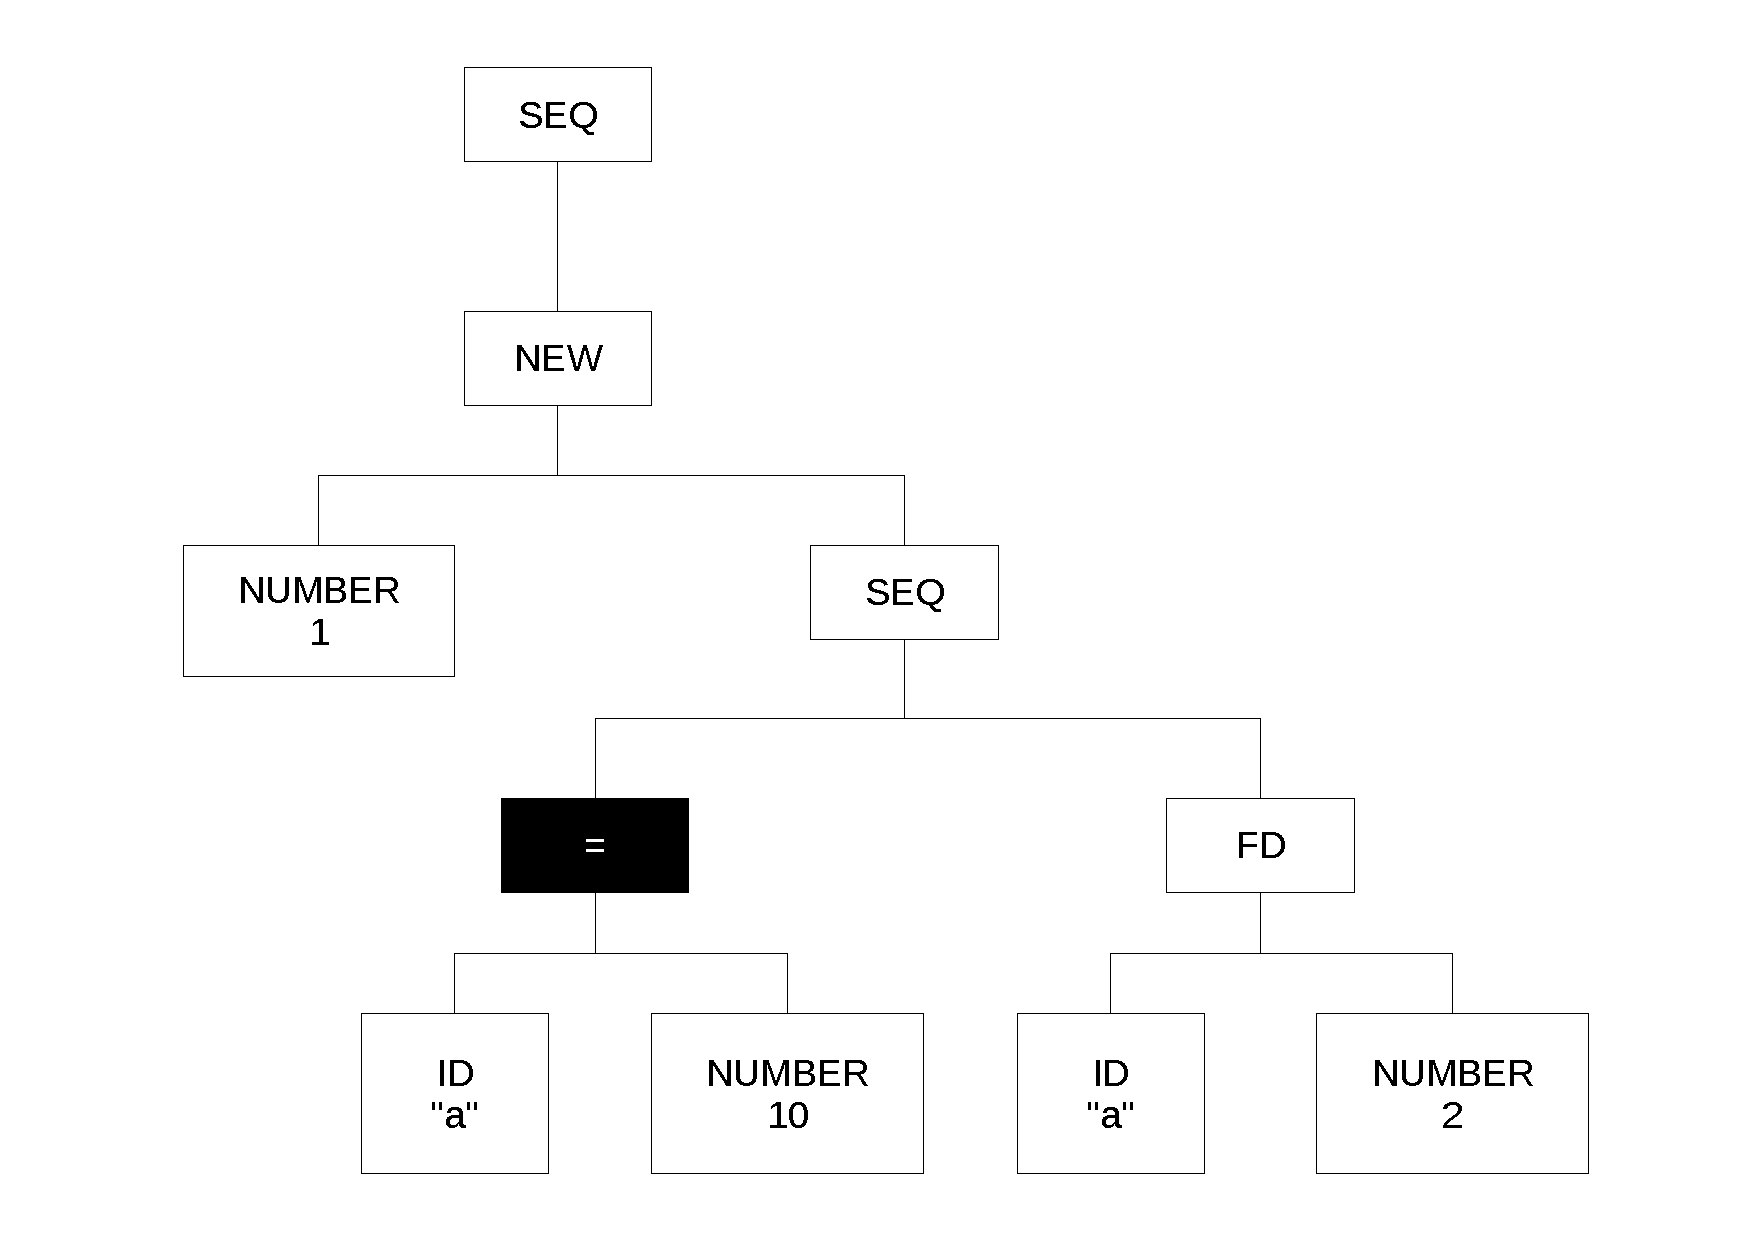
\includegraphics[scale=0.3]{doc/Presentation/img/arbre4.pdf}
\end{frame}

\begin{frame}
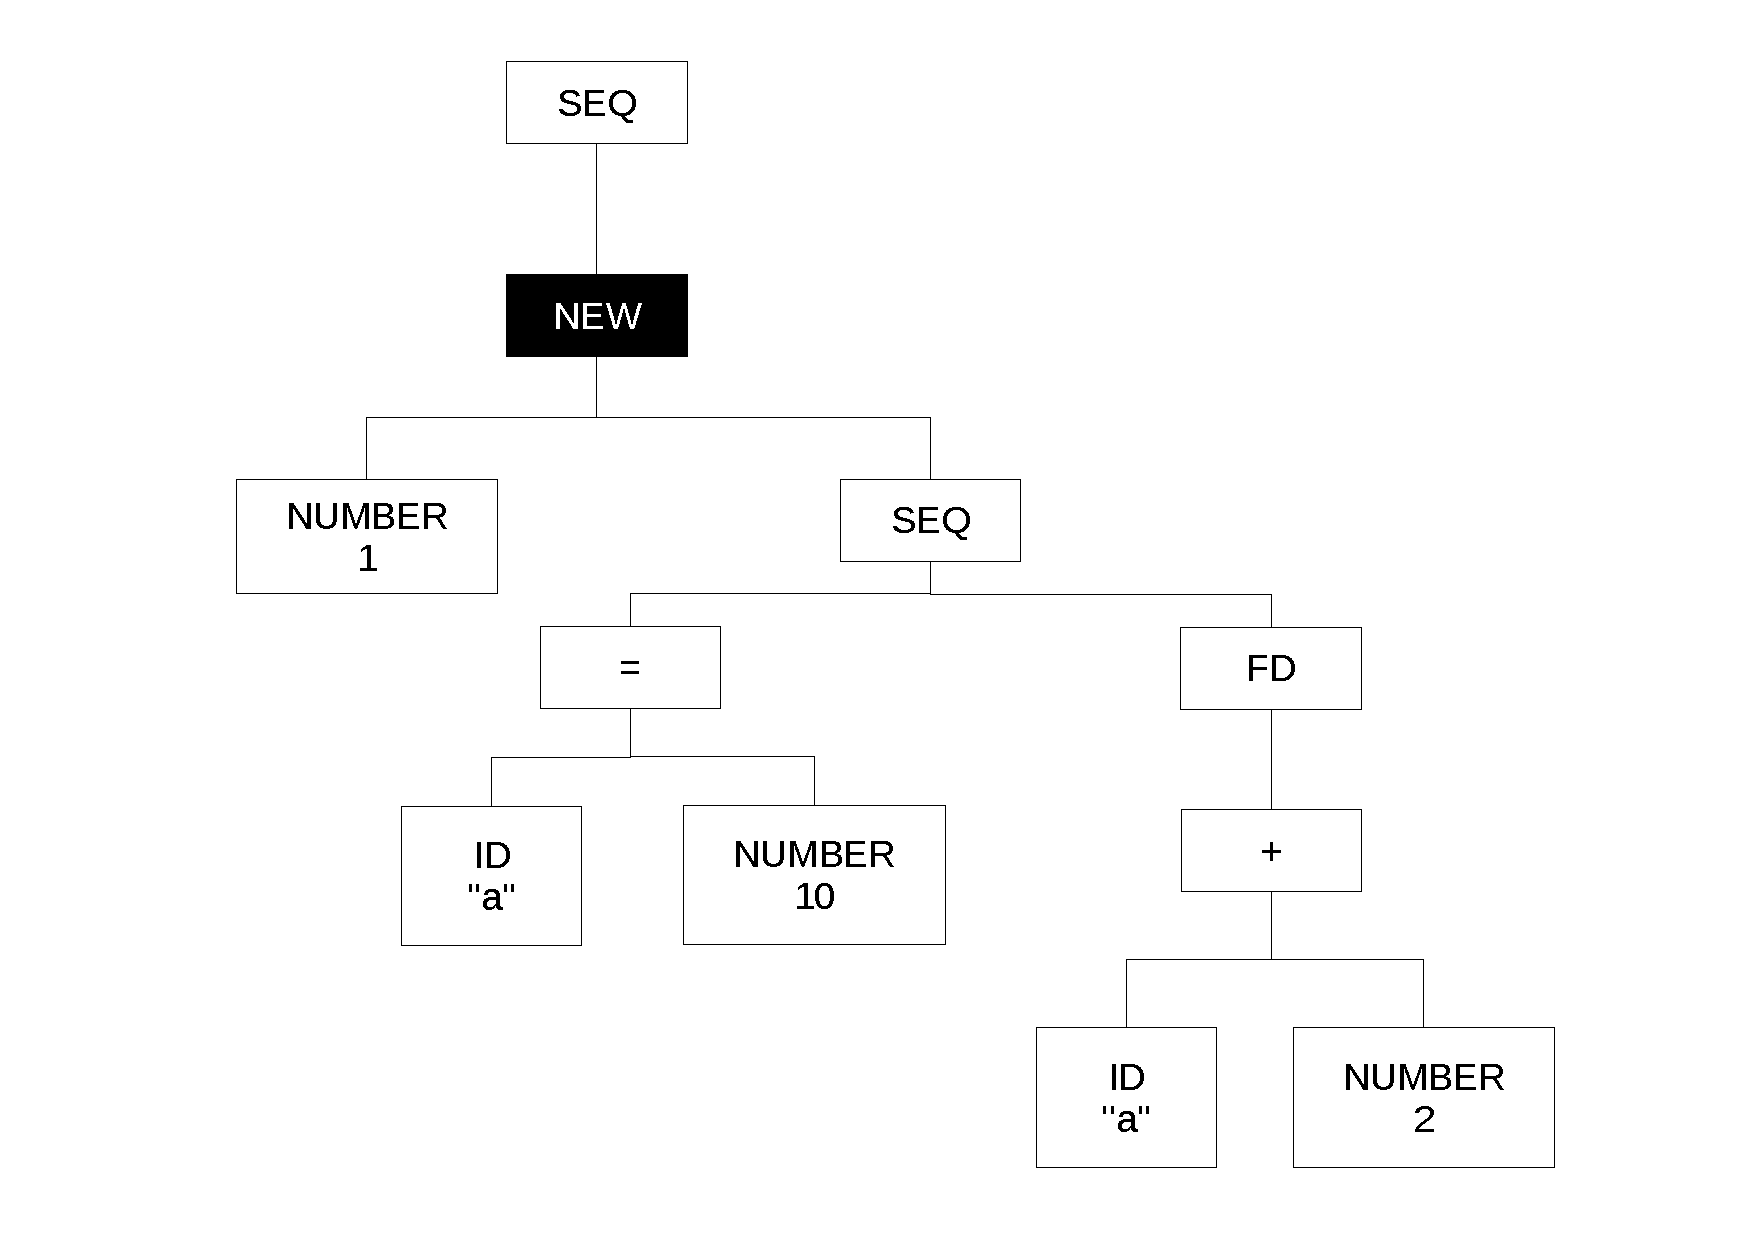
\includegraphics[scale=0.3]{doc/Presentation/img/arbre2.pdf}
\end{frame}

\begin{frame}
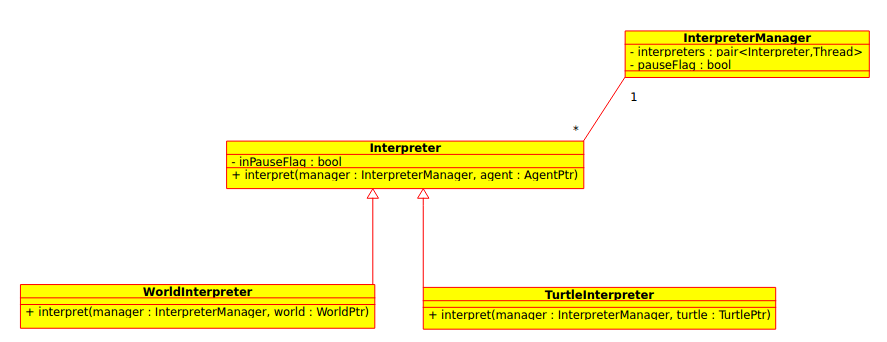
\includegraphics[scale=0.3]{doc/report/uml/interpreterUML.png}
\end{frame}

\begin{frame}
Rôle de l'interprète manager~:
\begin{itemize}
	\item Alerter des éventuelles pauses~;
	\item Création d'un monde avec les directives choisies~;
	\item Gérer les interpréteurs existants~;
	\item Stocker les couples threads-interprete créés.
\end{itemize}
C'est une sorte de gestionnaire d'interpréteurs.
\end{frame}

\begin{frame}
Un interprète~:
\begin{itemize}
	\item Analyse le jeton~;
	\item Effectue les analyses des enfants du noeud courant~;
	\item Appel la méthode correspondante dans le modèle.
\end{itemize}
\end{frame}
